%        File: report.tex
%     Created: Fri Jun 01 11:00 AM 2018 C
% Last Change: Fri Jun 01 11:00 AM 2018 C
%
\documentclass[a4paper]{article}
\usepackage{cite, graphicx, subfig, amsmath}
\usepackage[a4paper,top=3cm,bottom=4cm,right=3cm,left=3cm]{geometry}
\usepackage{siunitx}
\usepackage{indentfirst}

% For better navigation
\usepackage[hidelinks]{hyperref}
% For forcing image position (by using [H])
\usepackage{float}
% Need that just for \abs{}
\usepackage{physics}

\begin{document}
\title{Image Processing and Evaluation of Image Quality}
\author{Federico Battisti, Massimiliano Galli}
\date{June $2^{nd}$, 2018}
\maketitle

\begin{abstract}
	This is a report for the third laboratory session for the Applied Physics course, regarding image manipulation. The experience was structured into four main exercises:
	\begin{itemize}
		\item for the first exercise we were asked to reduce the noise present into 3 different images using operations both in the spacial and frequency domain, evaluating each time the quality of the pictures before and after the trasformation by means of signal to noise ratio (SNR) performed on a profile and on an extended area were the images were as uniform as possible;
    \item for the second exercise we had to perform a similar task on an image containing various parallel lines patterns at different frenquencies; exploiting this peculiarity we were also able to determine the spacial resolution in terms of Modulation Transfer Function (MTF) before and after the application of spacial and Fast Fourier Transform (FFT) noise reduction filters;
		\item for the third exercise we were asked to perform a flat-field correction on a mammographic image and evaluate, before and after, the image quality by means of SNR and Contrast-Noise Ratio (CNR);
    \item finally, using a phantom containing various framed circles at various diameters and levels of contrast, we were asked to calculate the CNR on each detail and graph that value as a function of the thickness of the detail.
	\end{itemize}
\end{abstract}

\clearpage

\section*{Exercise 1}
For the first part of the experience we were given three different pictures affected by different types of noise and artifacts created during acquisition by the acquisition devices themselves (Fig.~\ref{fig:ex_one}). We were then asked to perform operations both in the spatial and frequency domain in order to reduce the effect of the artifacts. In each situation we had to quantitatively verify the quality of the images before and after the operations performed by considering:
\begin{itemize}
 \item a profile on an almost uniform area and evaluating the background value by means of standard deviation from the mean grey level, which were both provided by ImageJ; a profile can be simply defined as a single line of pixels, the grey levels of which can be analyzed using the profile histogram option in ImageJ;
 \item Signal to Noise Ratio (SNR) on an almost uniform extended area , which can be defined as:
 \begin{equation}
 SNR=\frac{signal}{noise}=\frac{mean\ gray\ level}{gray\ level\ standard\ deviation}
 \end{equation}
 once again both the values can be obtained using the ImageJ options.
\end{itemize}

\begin{table}[h]
	\centering
	\begin{tabular}{| l | l | l | l |}
		\hline
		Figure & Operation & $\sigma_{profile}$ & SNR \\ \hline
		1a & raw & 6.78 & 11.12 \\ \hline
		1b & median filter & 3.65 & 23.33 \\ \hline
		2a & low-pass filter & 3.65 & 24.60 \\ \hline
		1c & raw & 7.45 & 10.28 \\ \hline
		1d & mean filter & 4.90 & 16.54 \\ \hline
		2c & low-pass filter & 5.37 & 16.03 \\ \hline
		1e & raw & 77.97 & 0.77 \\ \hline
		1f & gaussian filter & 1.78 & 35.28 \\ \hline
		2e & low-pass filter & 7.86 & 5.45 \\ \hline
	\end{tabular}
  \caption{Noise and SNR values for the three images before and after the transforms. We can see that for every image the noise decreases and consequently the SNR encreases.}
  \label{tab:ex_one}
\end{table}

In the spatial domain we decided to use a median filter for Fig.~\ref{kiddo_raw} , a mean filter for Fig.~\ref{tetta_raw} and a gaussian filter for Fig.~\ref{moon_raw}. As for the FFT operations we decided to apply a low-pass filter to all three of the images, in order to cut all the high frequencies from the frequency domain, since our objective was to reduce noise. The results of these operations can be seen in Fig.~\ref{fig:ex_one} and \ref{fig:ex_one_fft} respectively, while the profile standard deviation and the SNR for the extended area for each picture and each transformation are reported in Tab. \ref{tab:ex_one}.

As it was to be expected the noise reduction operations managed to reduce the profile standard deviation and augment the SNR which are both signs of improvement in image quality.

\begin{figure}[!htb]
  \centering
  \subfloat[][]{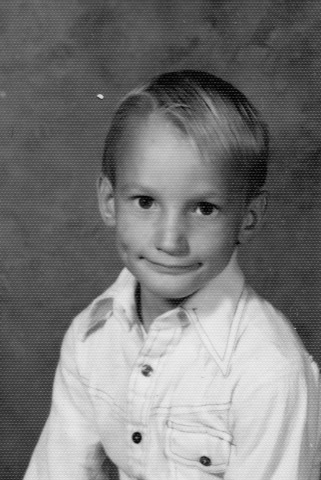
\includegraphics[width=.35\textwidth]{./immagini_terza_prova/kiddo.png}\label{kiddo_raw}}\quad
  \subfloat[][]{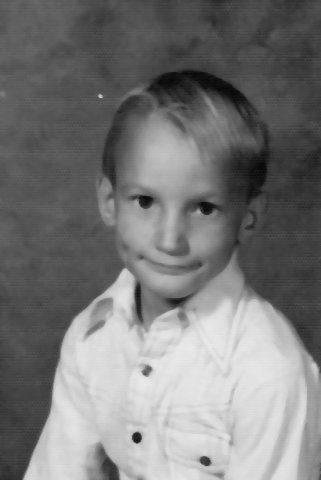
\includegraphics[width=.35\textwidth]{./immagini_terza_prova/kiddo_1/kiddo_median.jpg}\label{kiddo_median}}\\
  \subfloat[][]{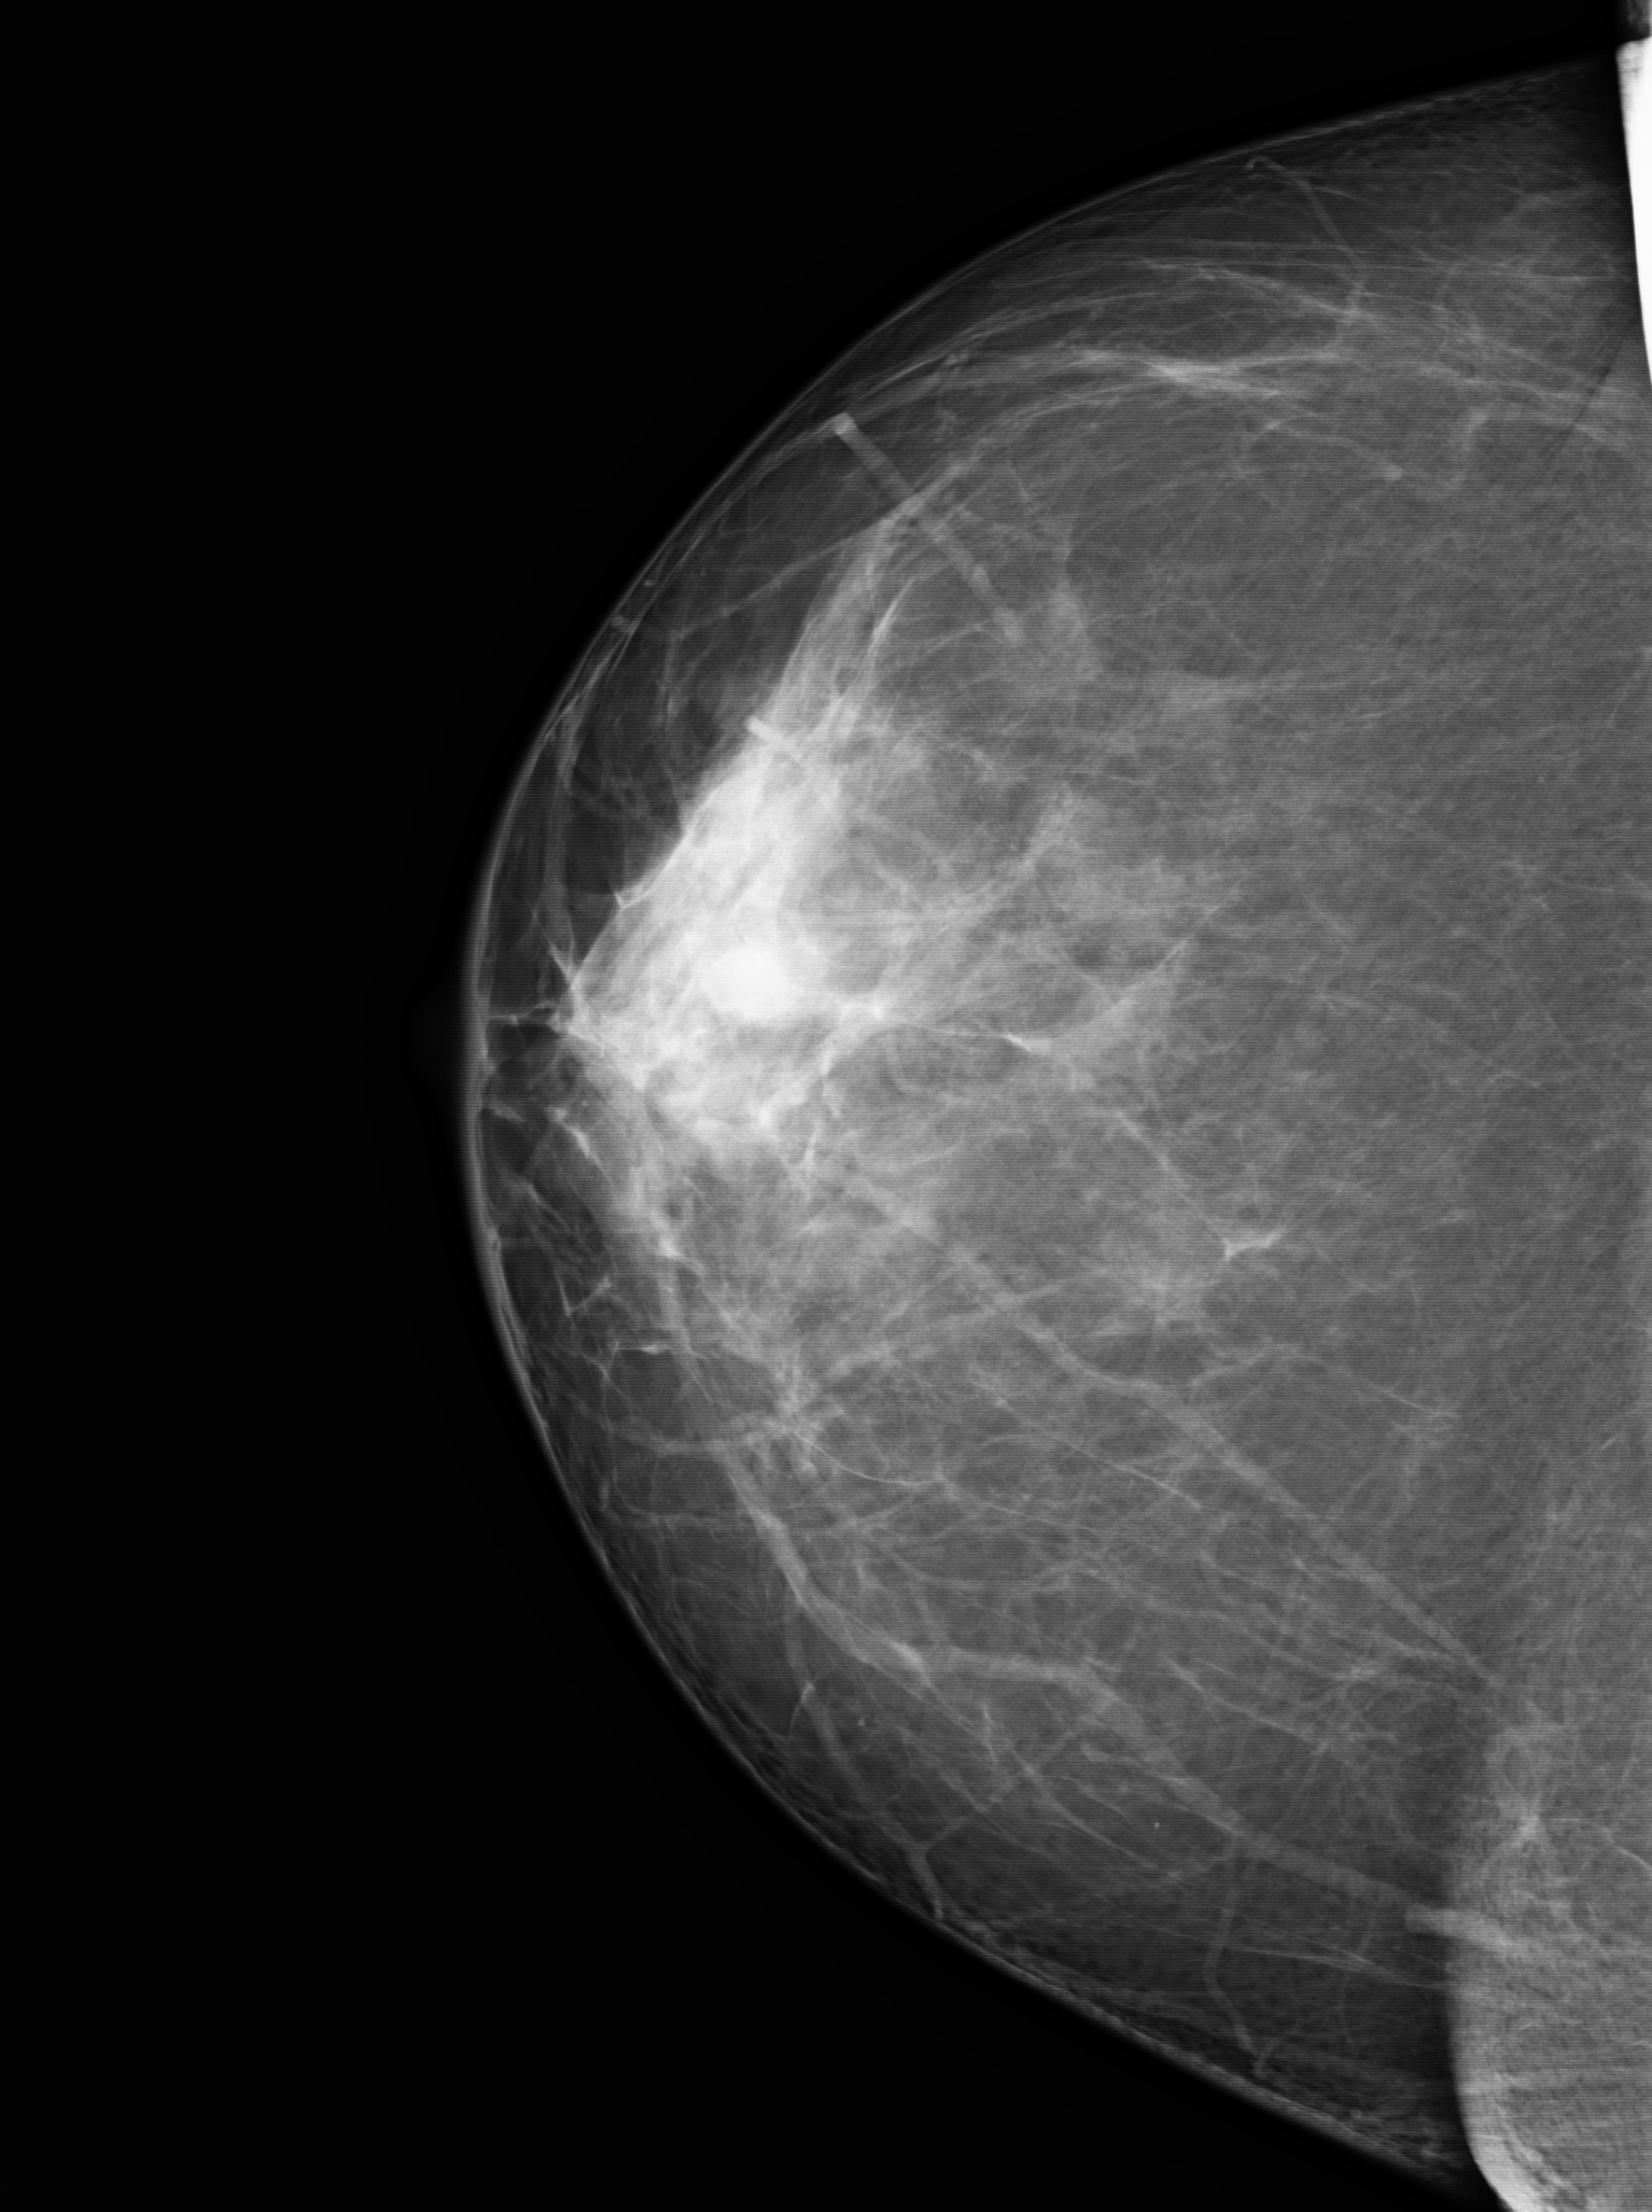
\includegraphics[width=.35\textwidth]{./immagini_terza_prova/griglia_mammo.png}\label{tetta_raw}}\quad
  \subfloat[][]{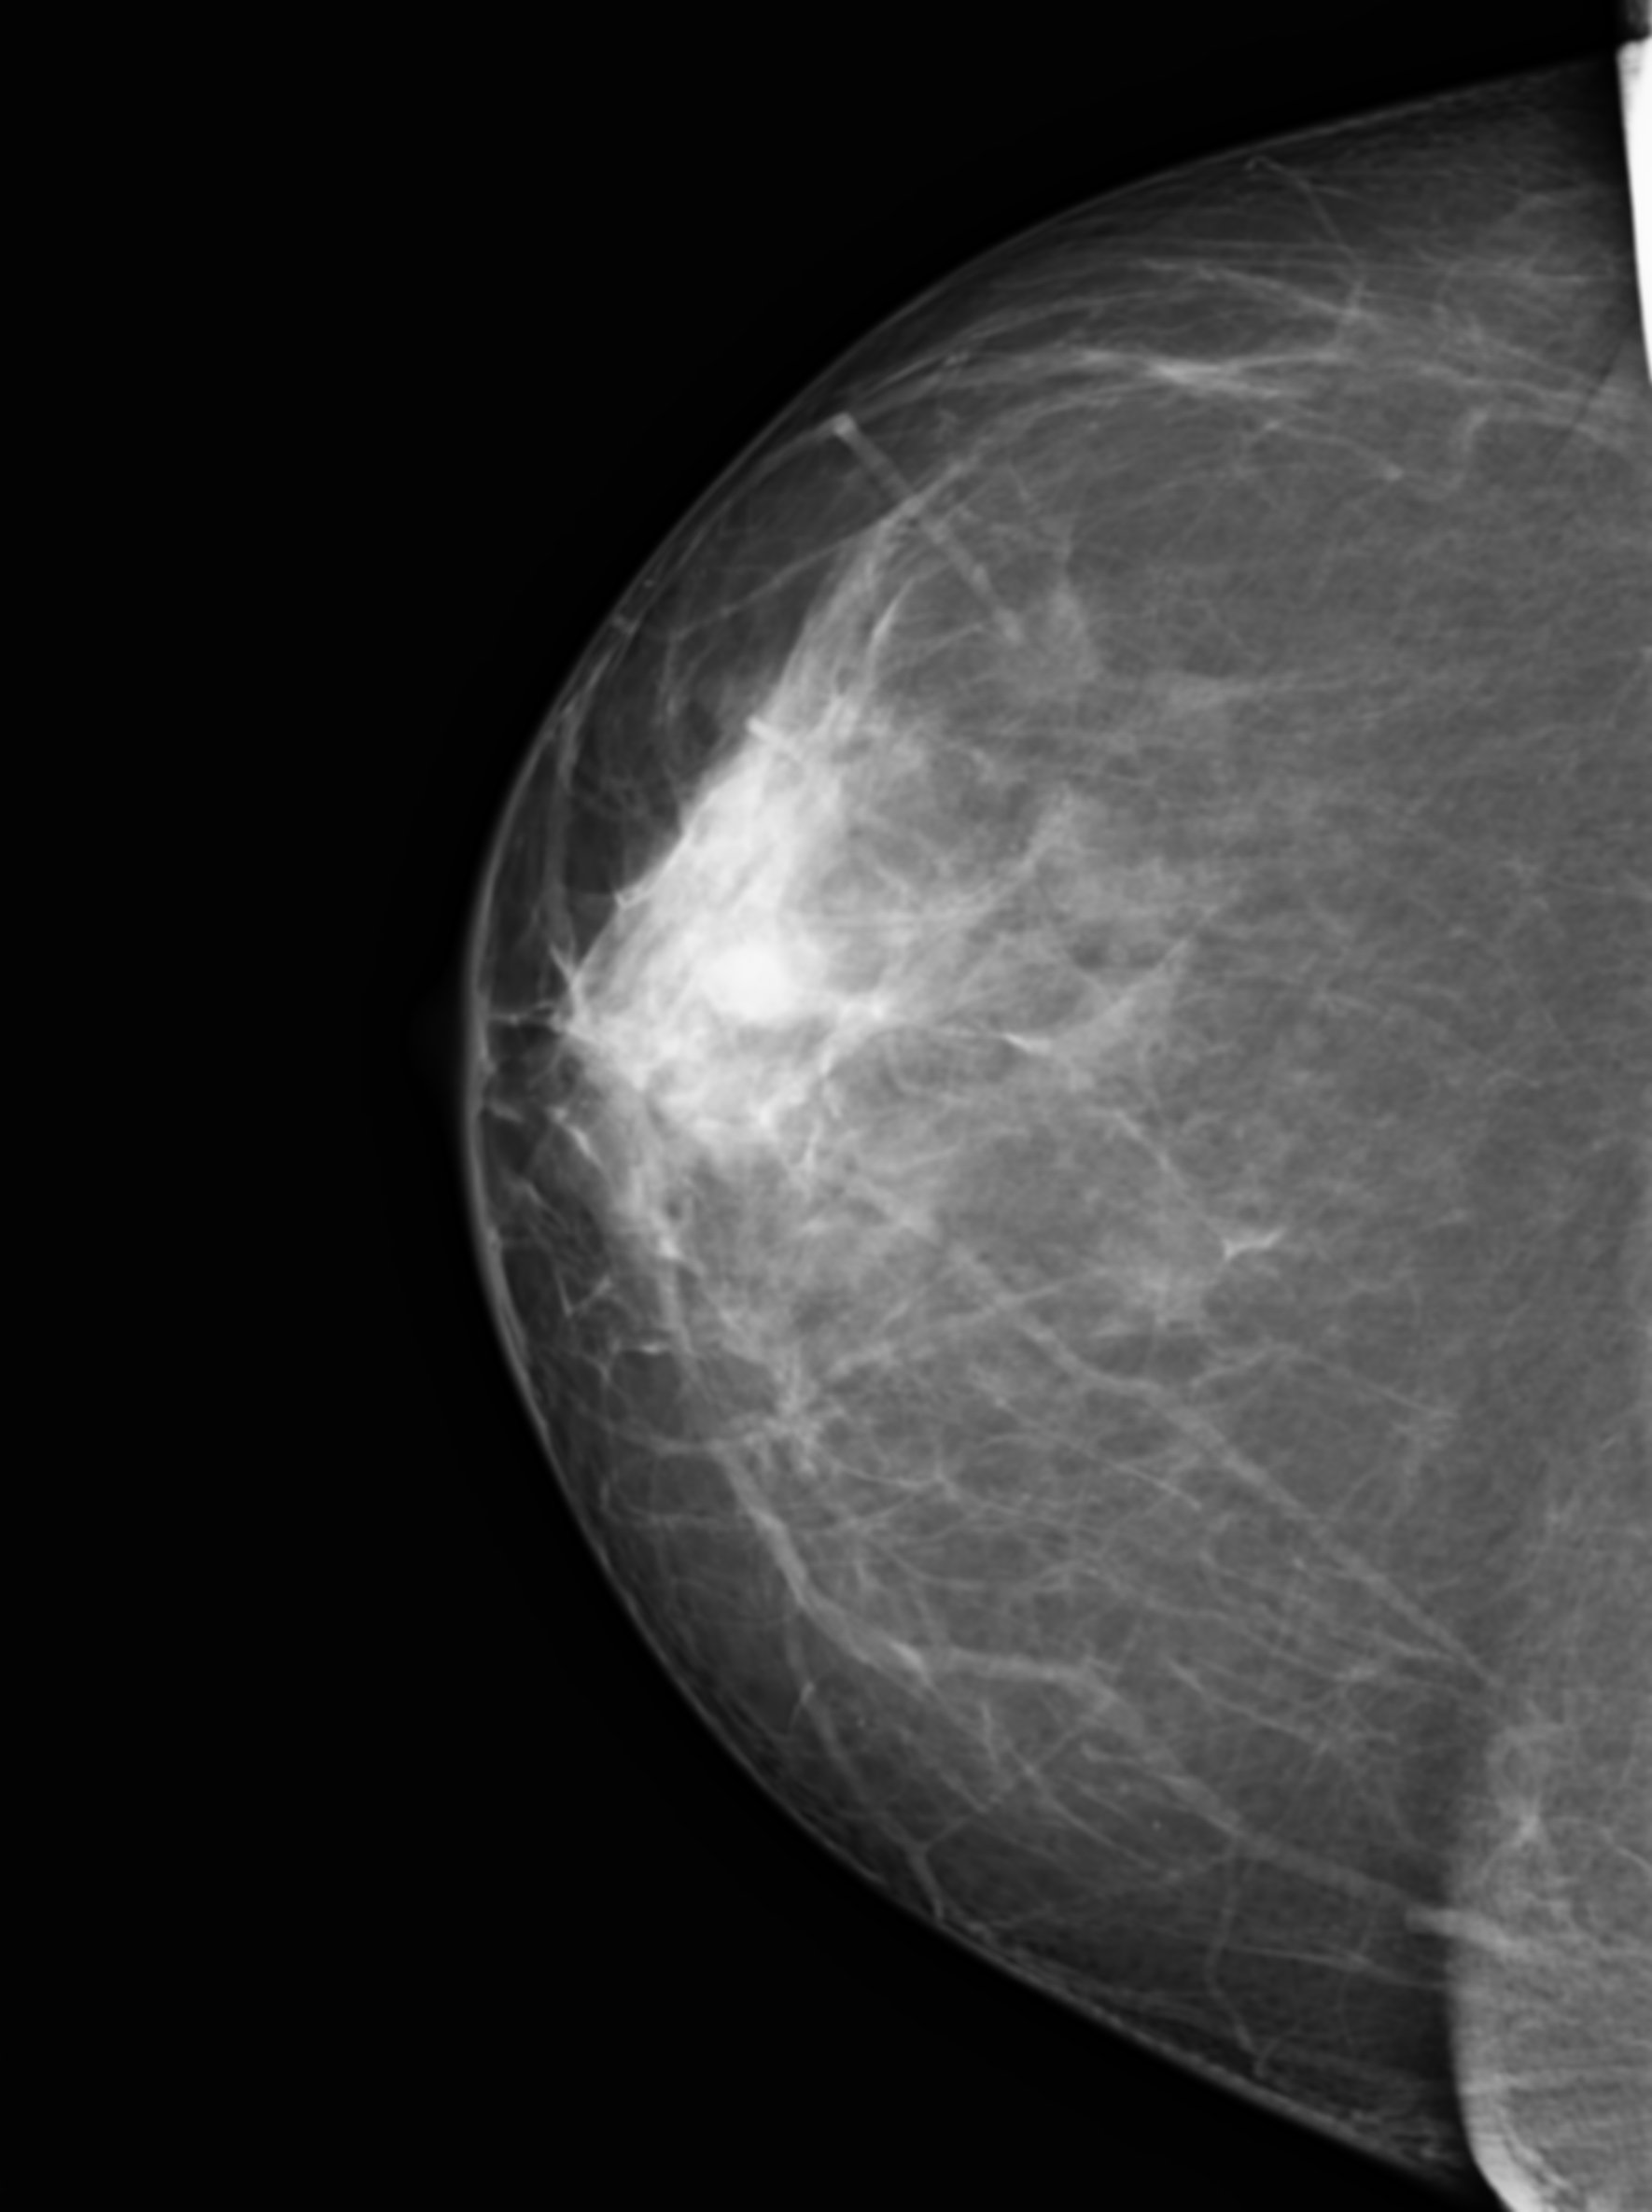
\includegraphics[width=.35\textwidth]{./immagini_terza_prova/tetta_1/tetta_mean.jpg}\label{tetta_mean}}\\
  \subfloat[][]{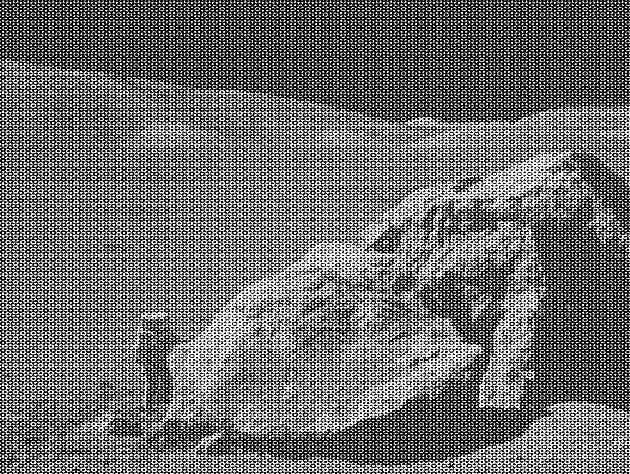
\includegraphics[width=.35\textwidth]{./immagini_terza_prova/moonlanding.png}\label{moon_raw}}\quad
  \subfloat[][]{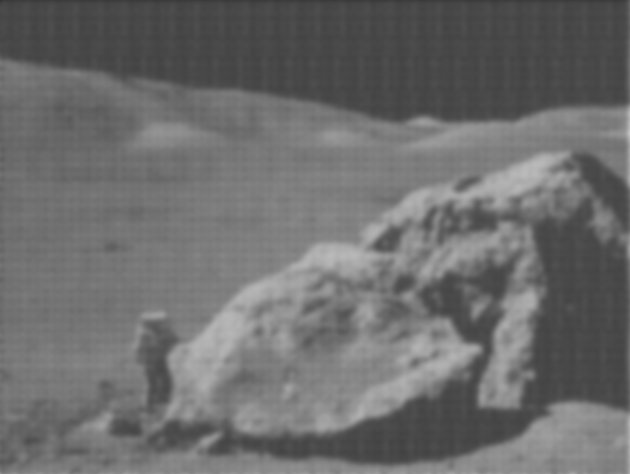
\includegraphics[width=.35\textwidth]{./immagini_terza_prova/moon_1/moonlanding_gauss.jpg}\label{moon_gaussian}}
  \caption{(a), (c), (e): pictures used in their raw form. (b): median transform of (a). (d): mean transform of (c). (f): gaussian transform of (e).}
  \label{fig:ex_one}
\end{figure}

\begin{figure}[!htb]
	\centering
  \subfloat[][]{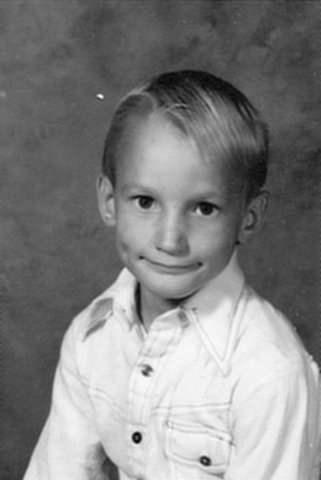
\includegraphics[height=2in]{./immagini_terza_prova/kiddo_1/kiddo_filtered_fft.jpg}}\quad
  \subfloat[][]{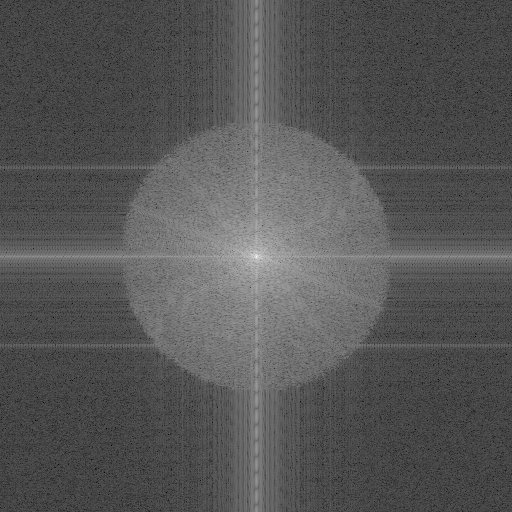
\includegraphics[height=2in]{./immagini_terza_prova/kiddo_1/FFTofkiddo_filtered_fft.jpg}}\\
  \subfloat[][]{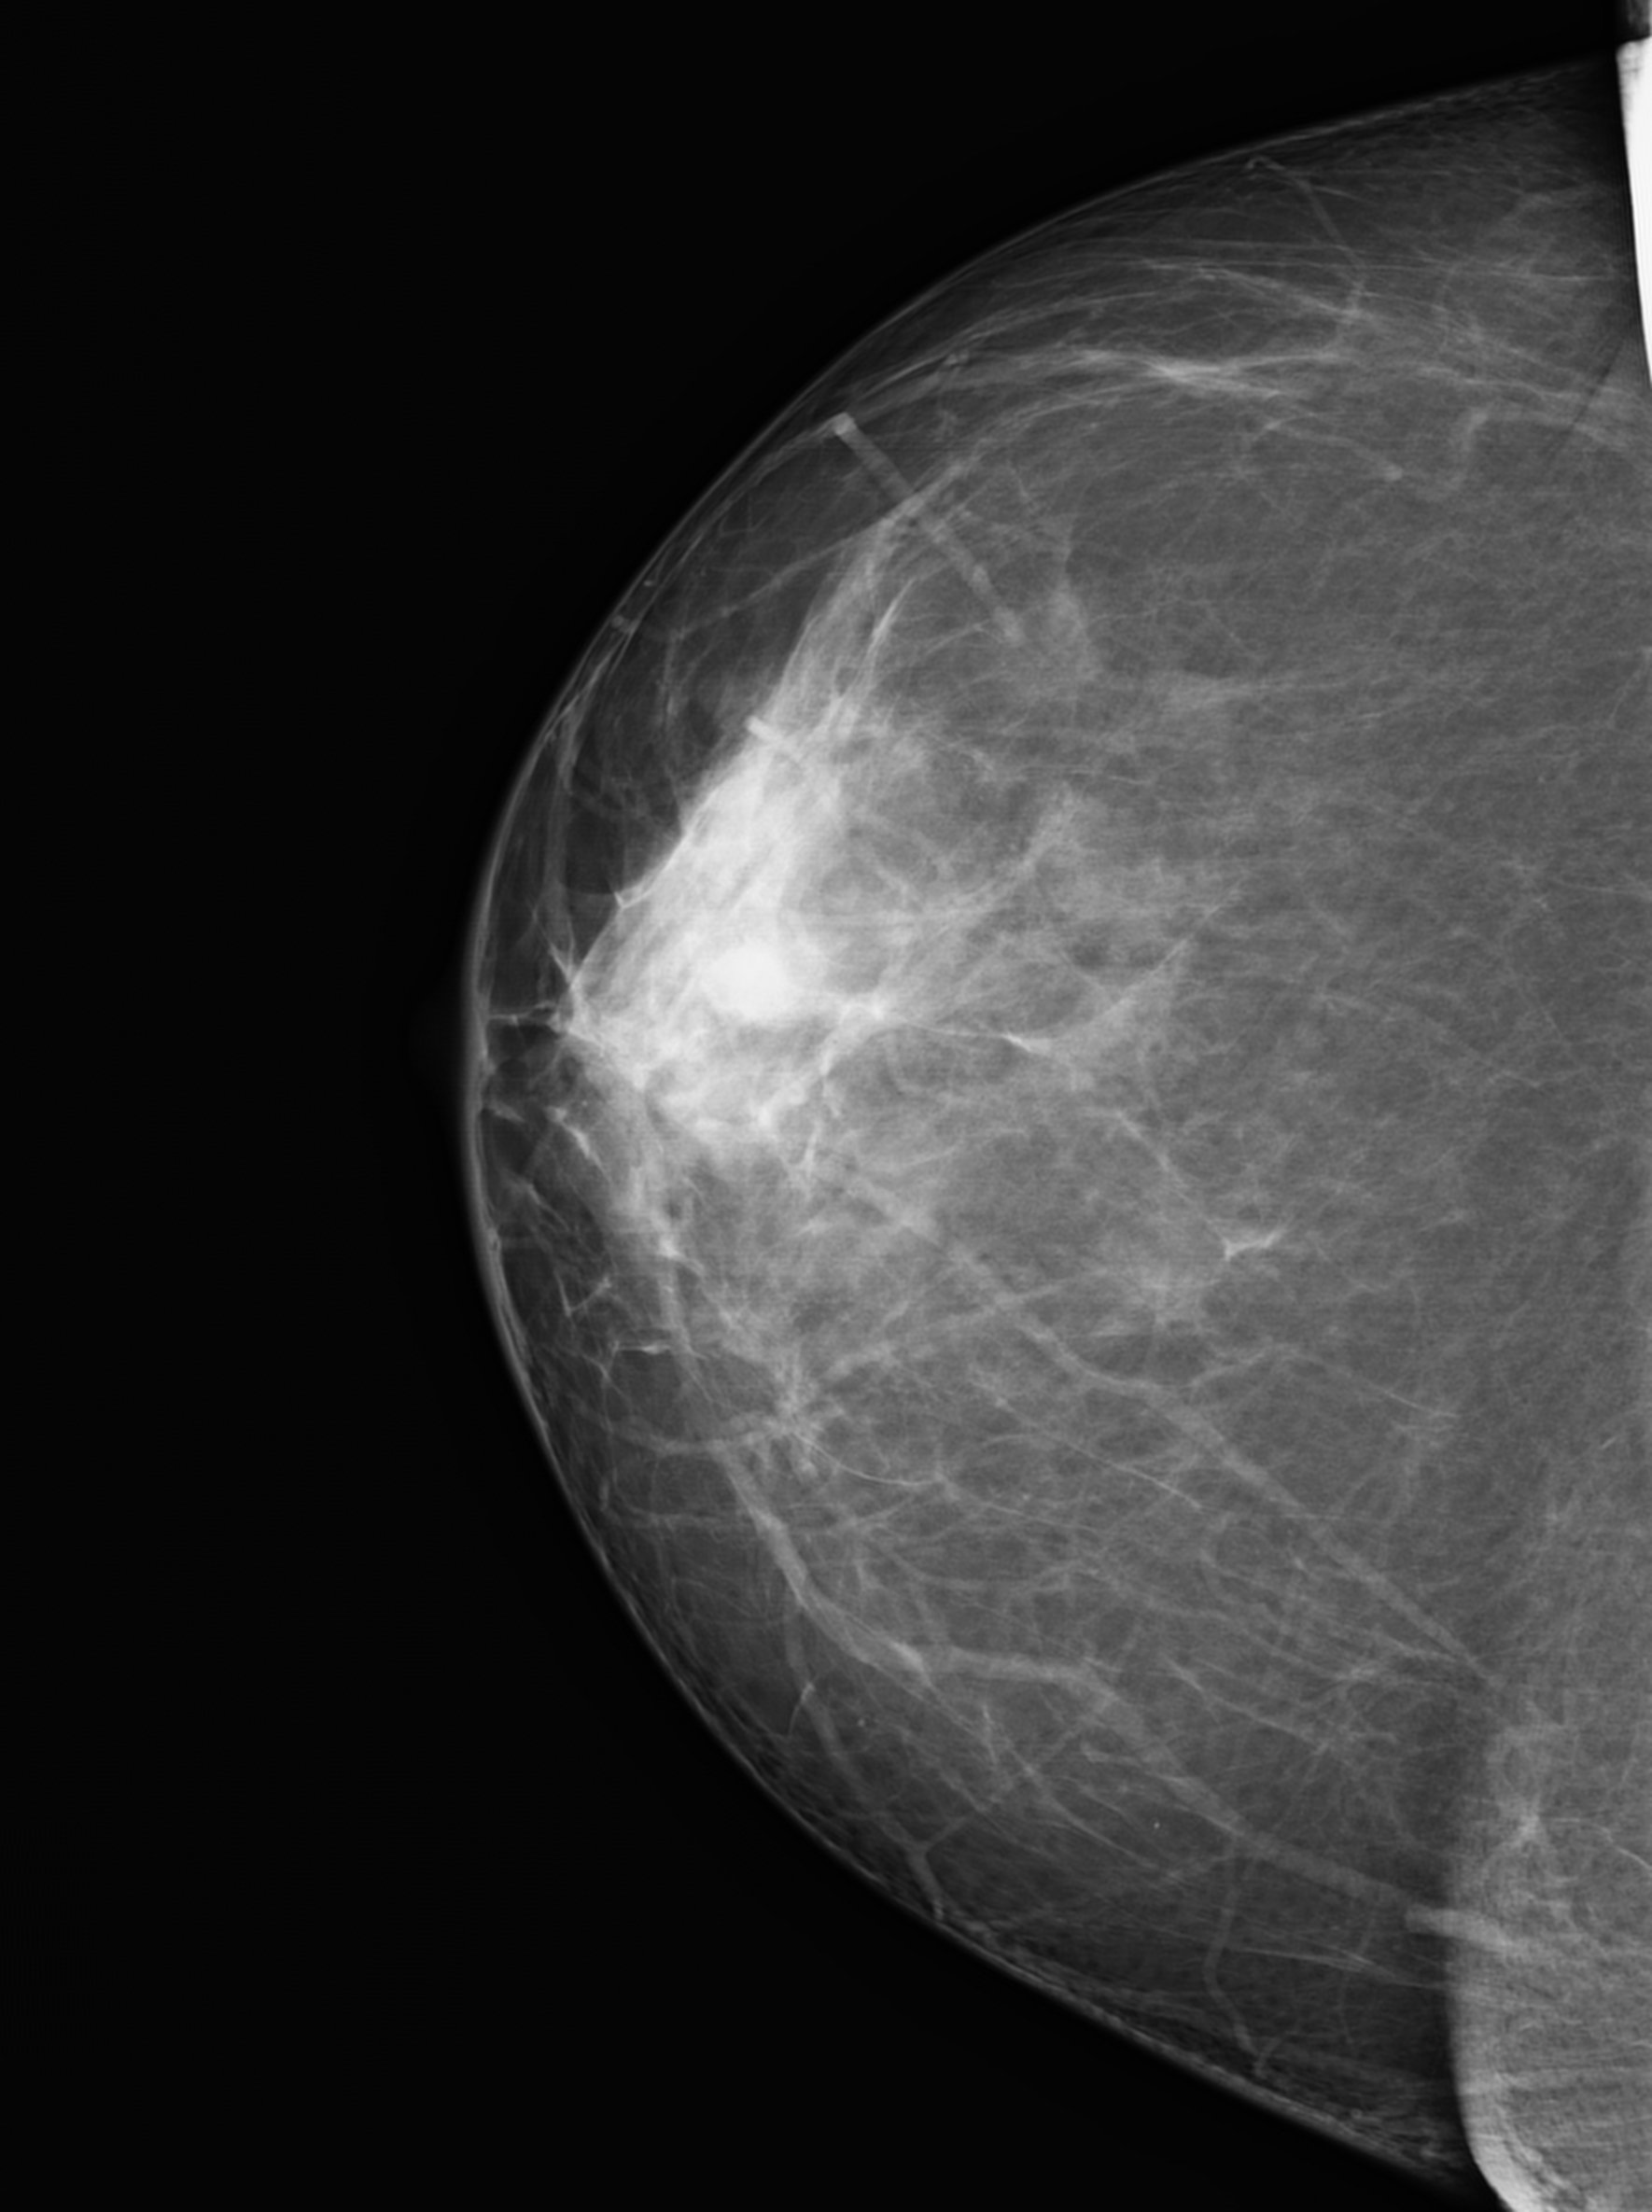
\includegraphics[height=2in]{./immagini_terza_prova/tetta_1/griglia_mammo_fft.jpg}}\quad
  \subfloat[][]{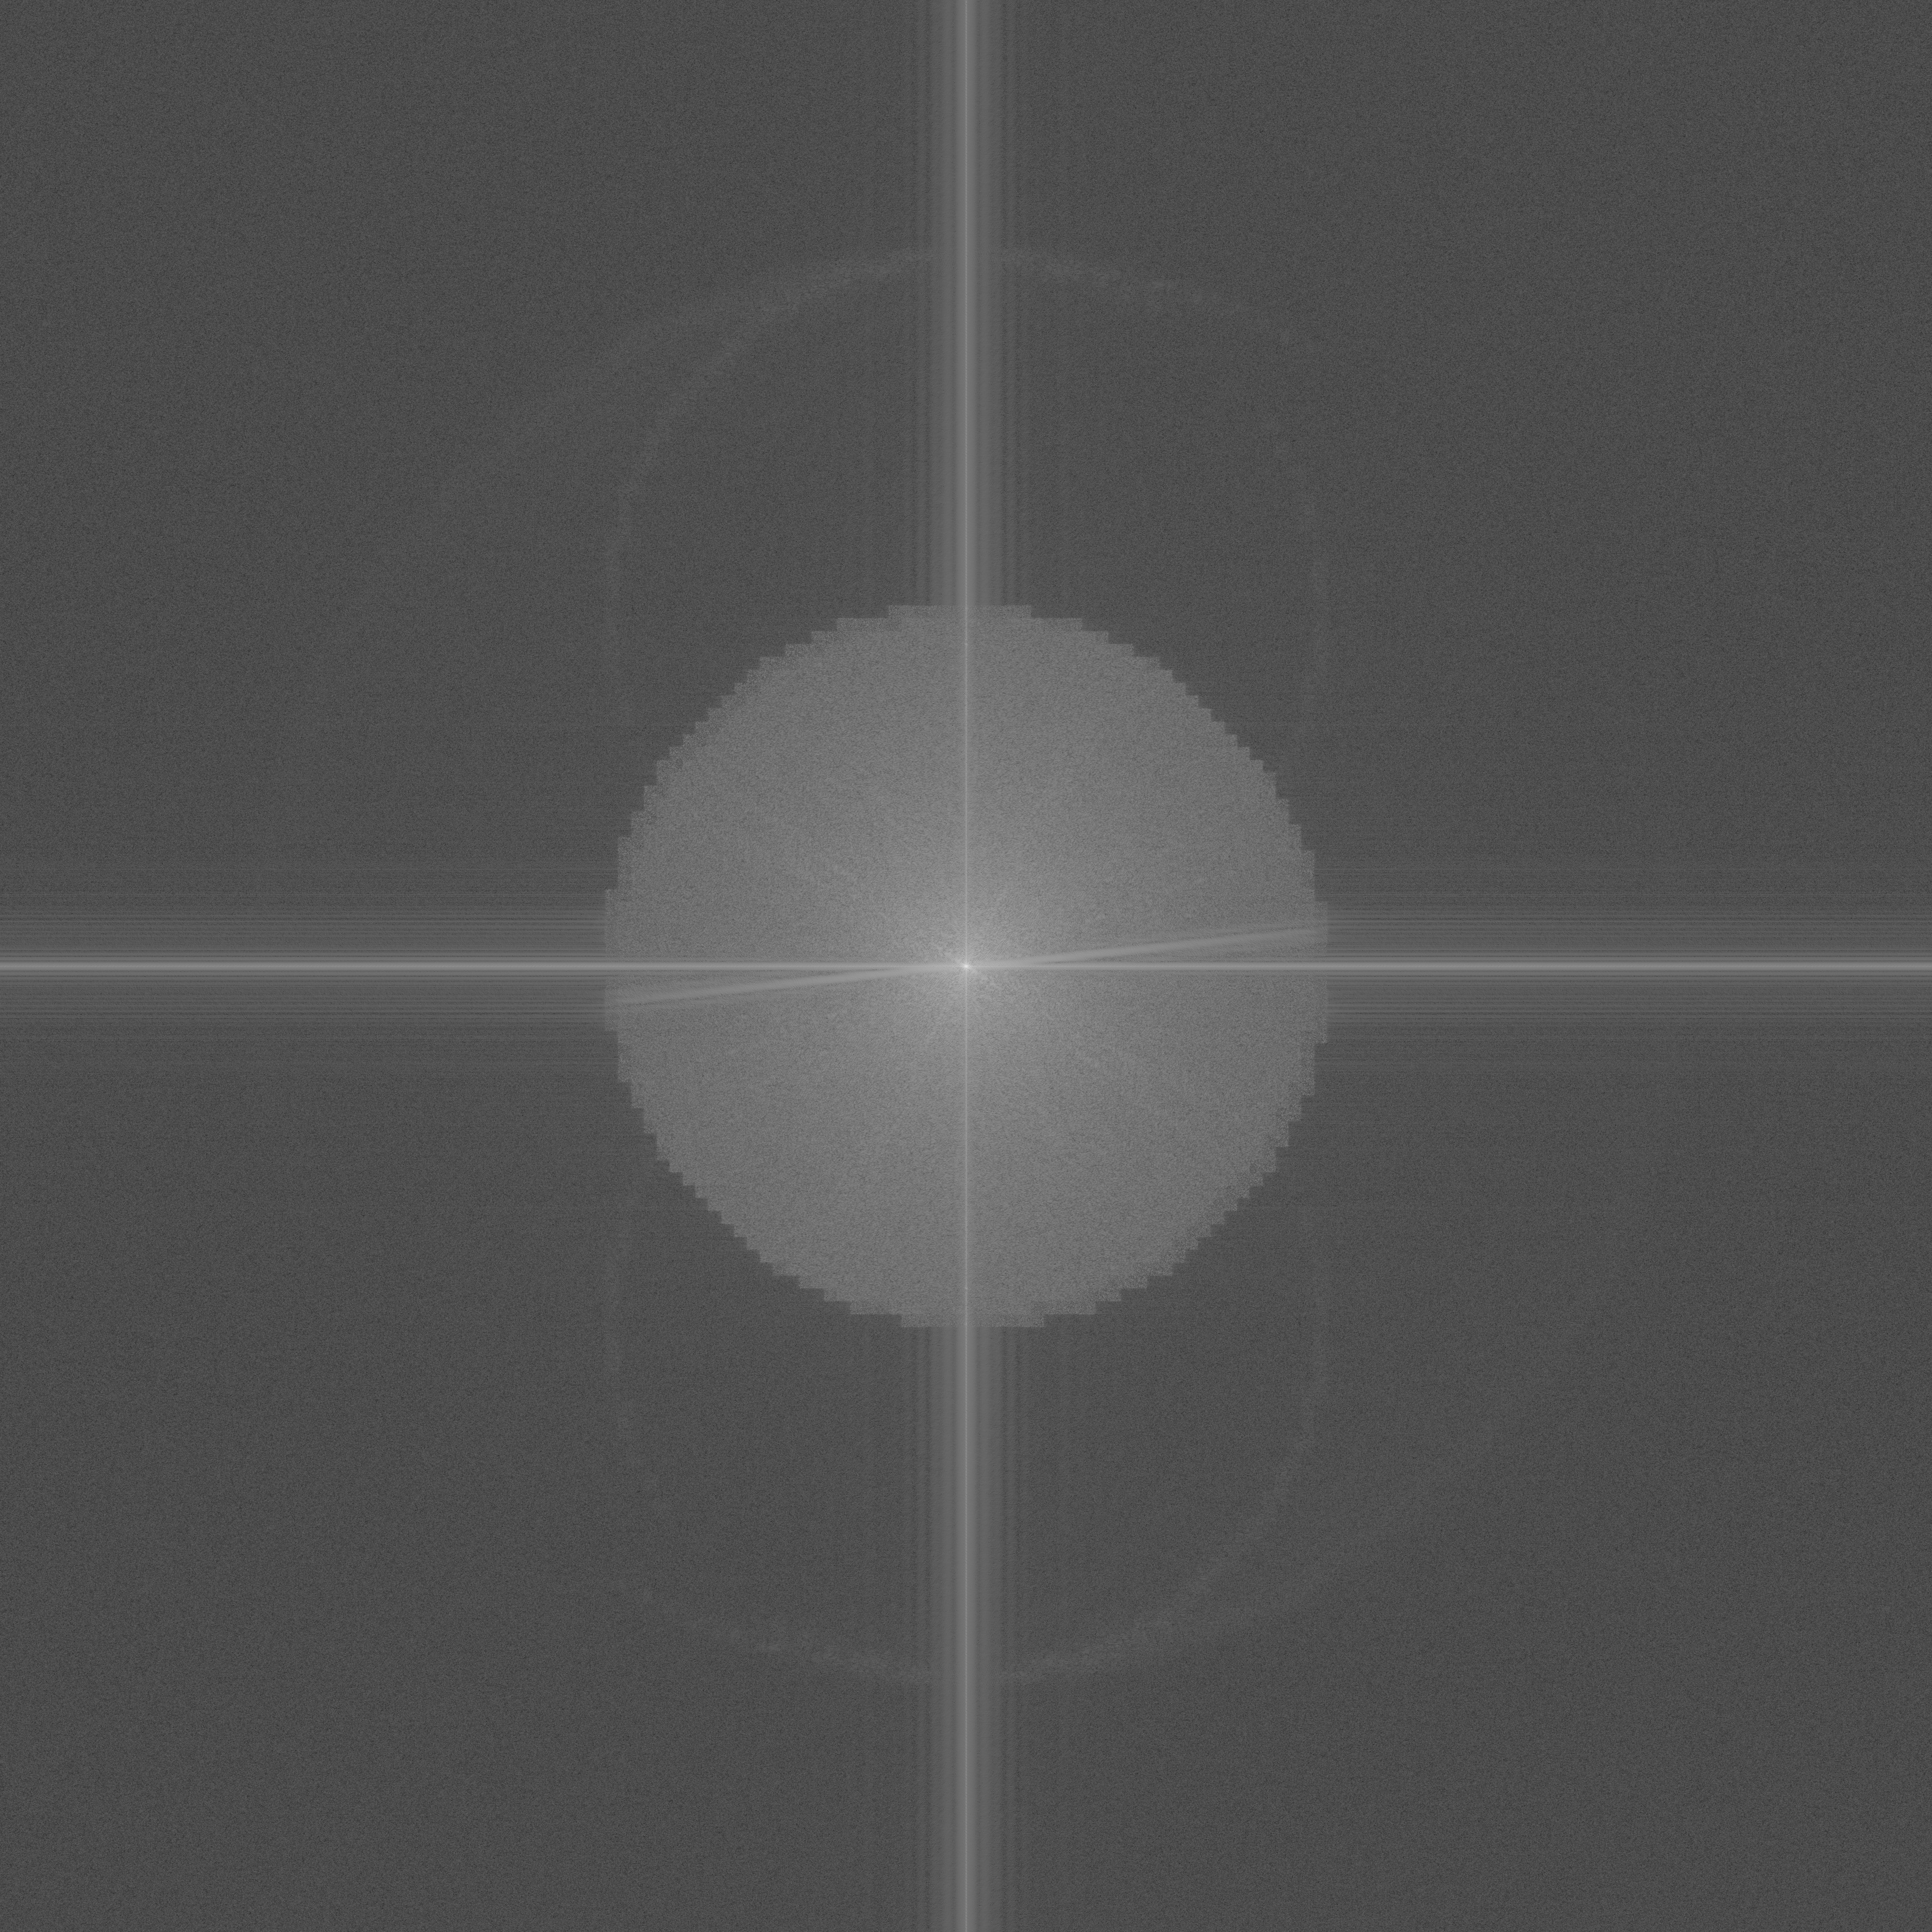
\includegraphics[height=2in]{./immagini_terza_prova/tetta_1/FFTofgriglia_mammo_fft.jpg}}\\
  \subfloat[][]{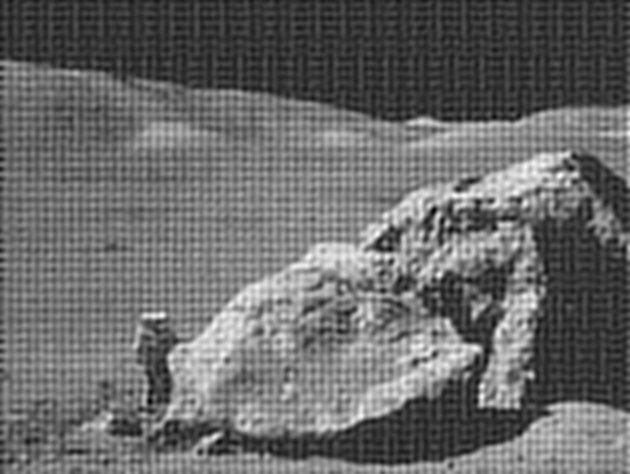
\includegraphics[height=2in]{./immagini_terza_prova/moon_1/moonlanding_fft.jpg}}\quad
  \subfloat[][]{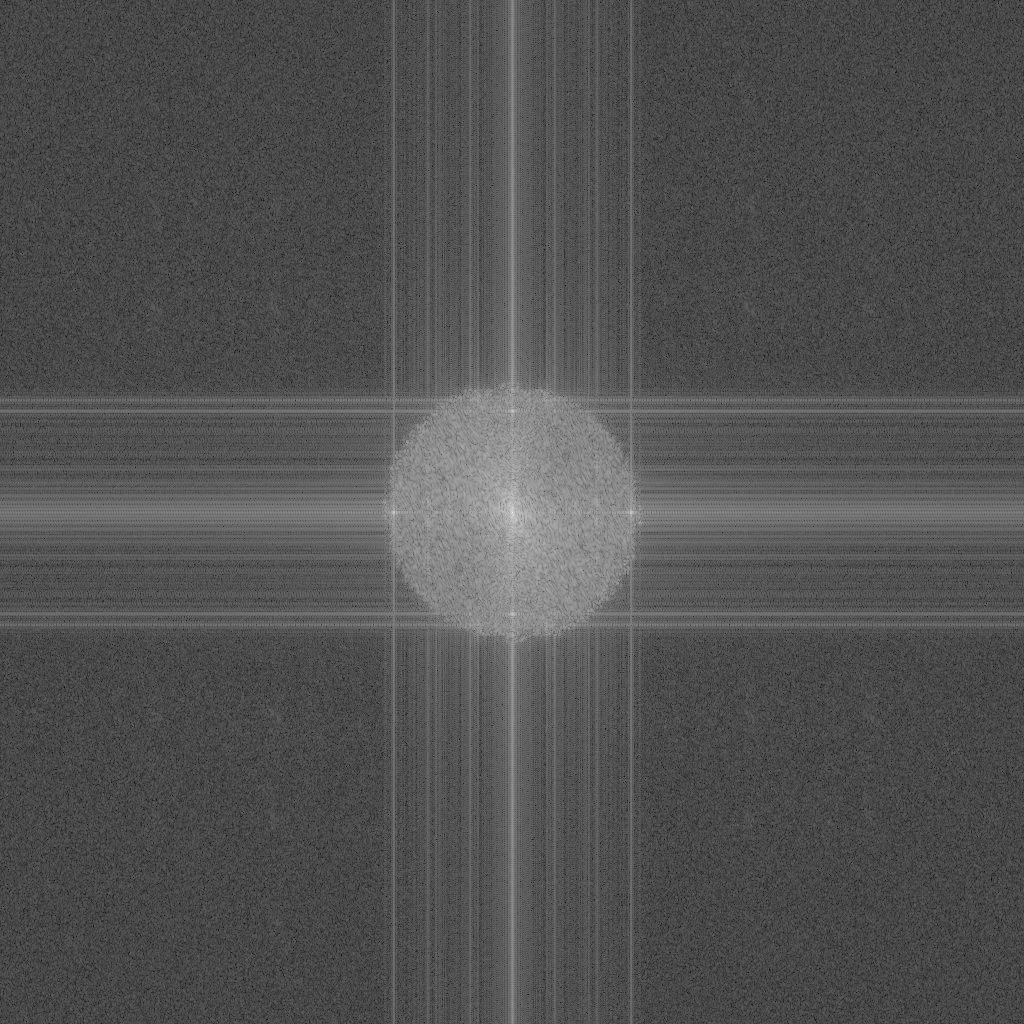
\includegraphics[height=2in]{./immagini_terza_prova/moon_1/FFTofmoonlanding_fft.jpg}}
	\caption{Pictures modified using low-pass frequency filters alongside their respective FFT domain.}
  \label{fig:ex_one_fft}
\end{figure}

\clearpage





\section*{Exercise 2}

\begin{figure}[!hbt]
  \centering
  \subfloat[][]{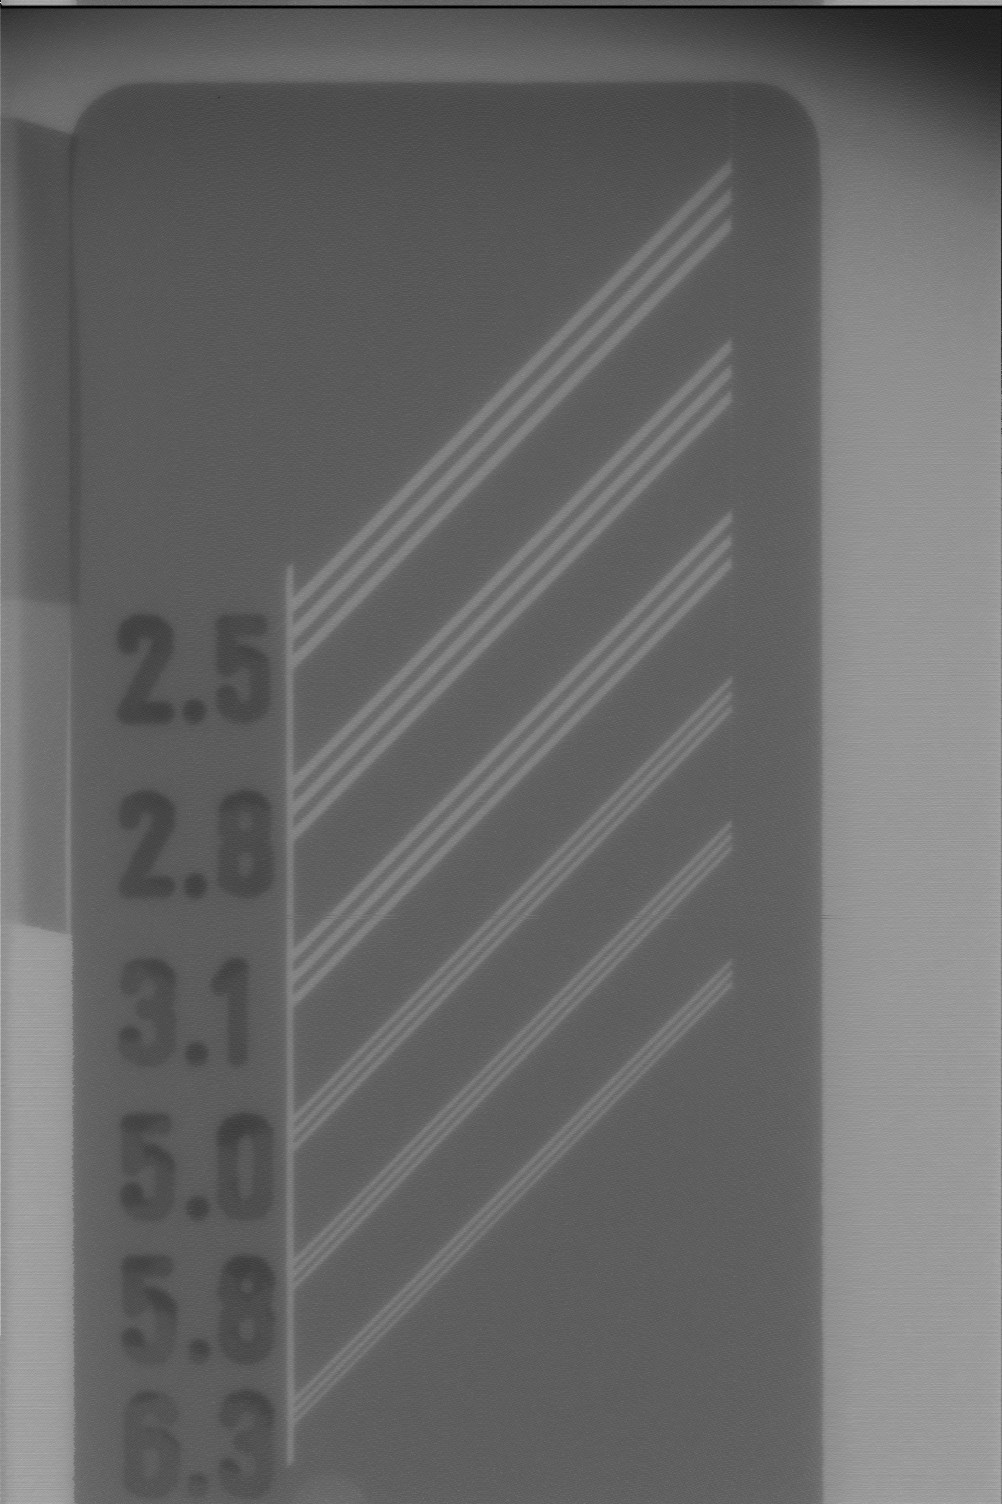
\includegraphics[width=.33\textwidth]{./immagini_terza_prova/ex2/raw0.jpg}\label{raw0}}\quad
  \subfloat[][]{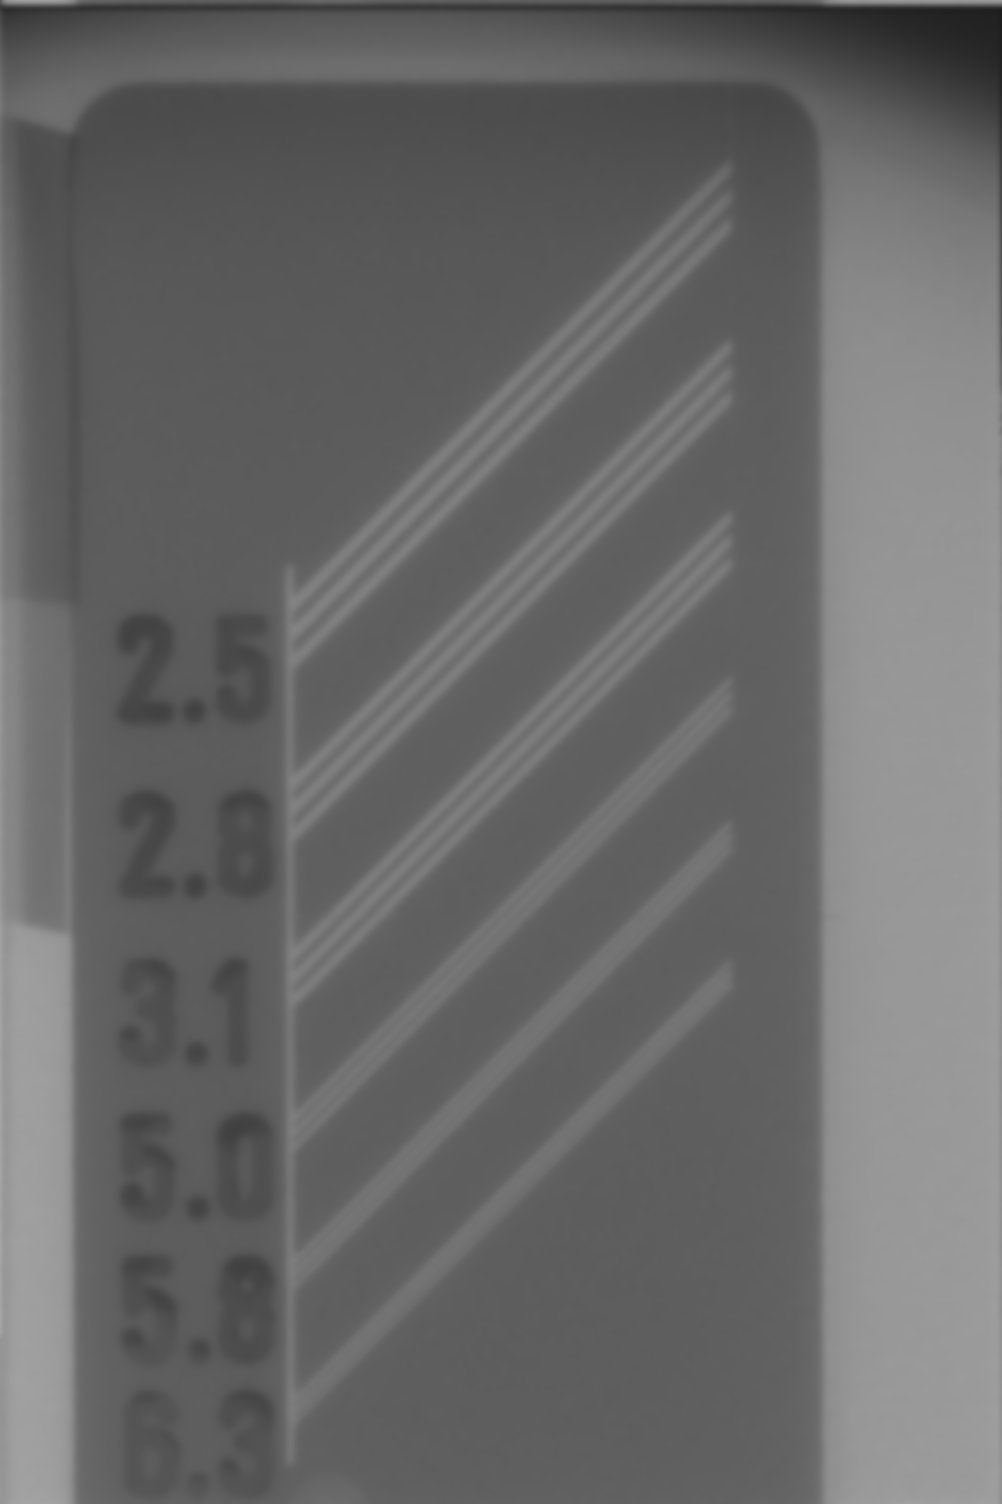
\includegraphics[width=.33\textwidth]{./immagini_terza_prova/ex2/gaussian.jpg}}\\
  \subfloat[][]{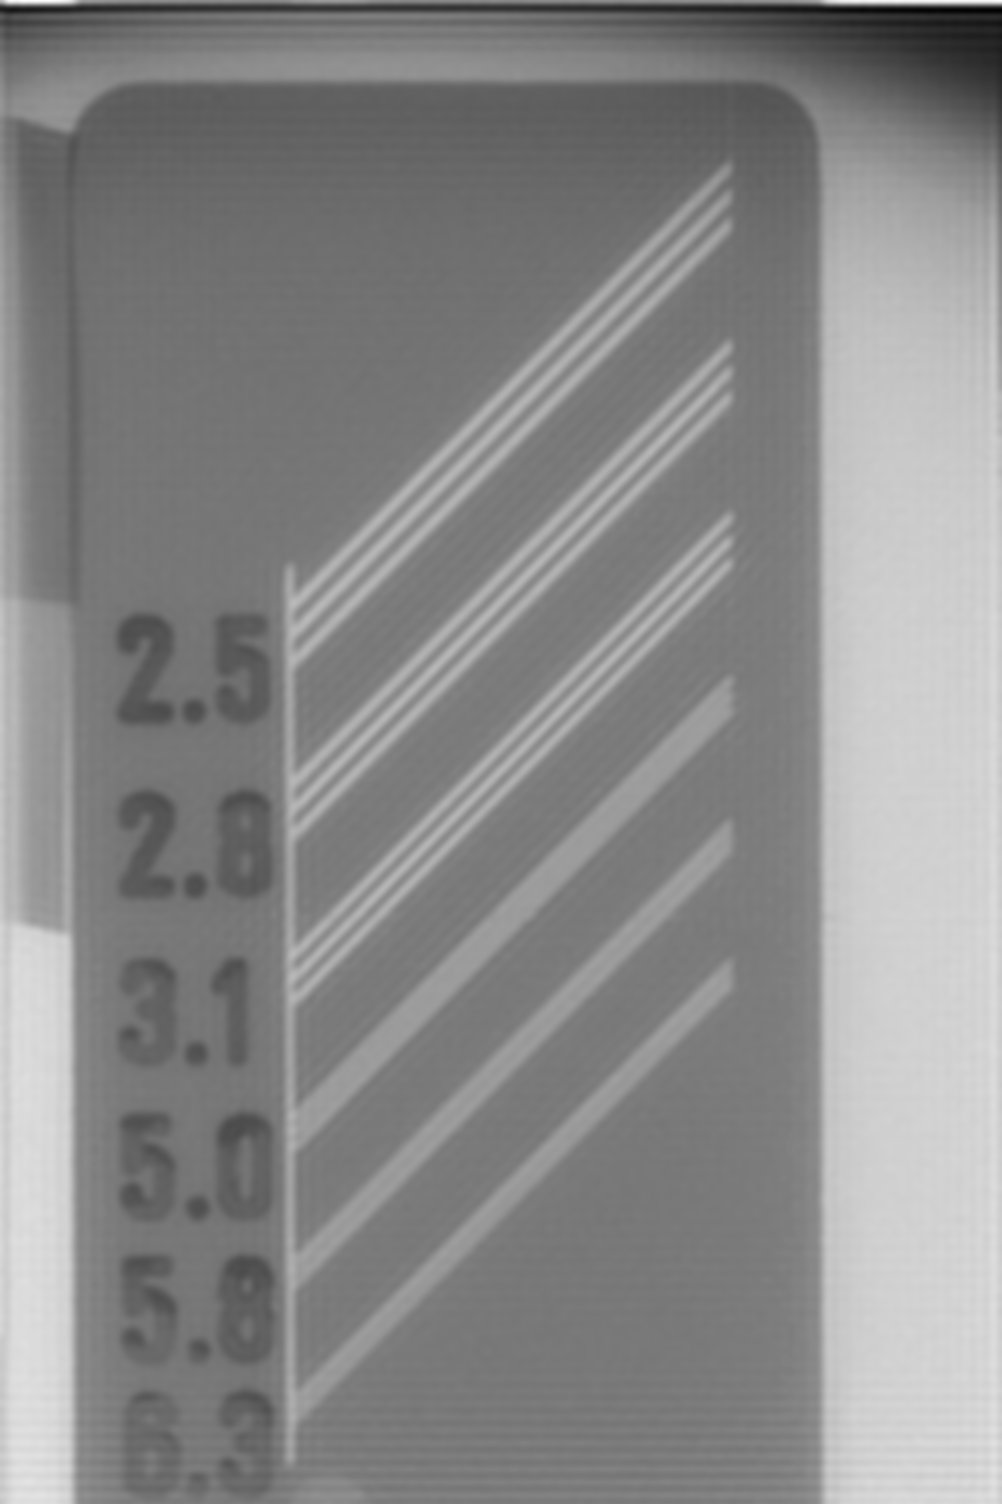
\includegraphics[height=2in]{./immagini_terza_prova/ex2/raw0_fft.jpg}}\quad
  \subfloat[][]{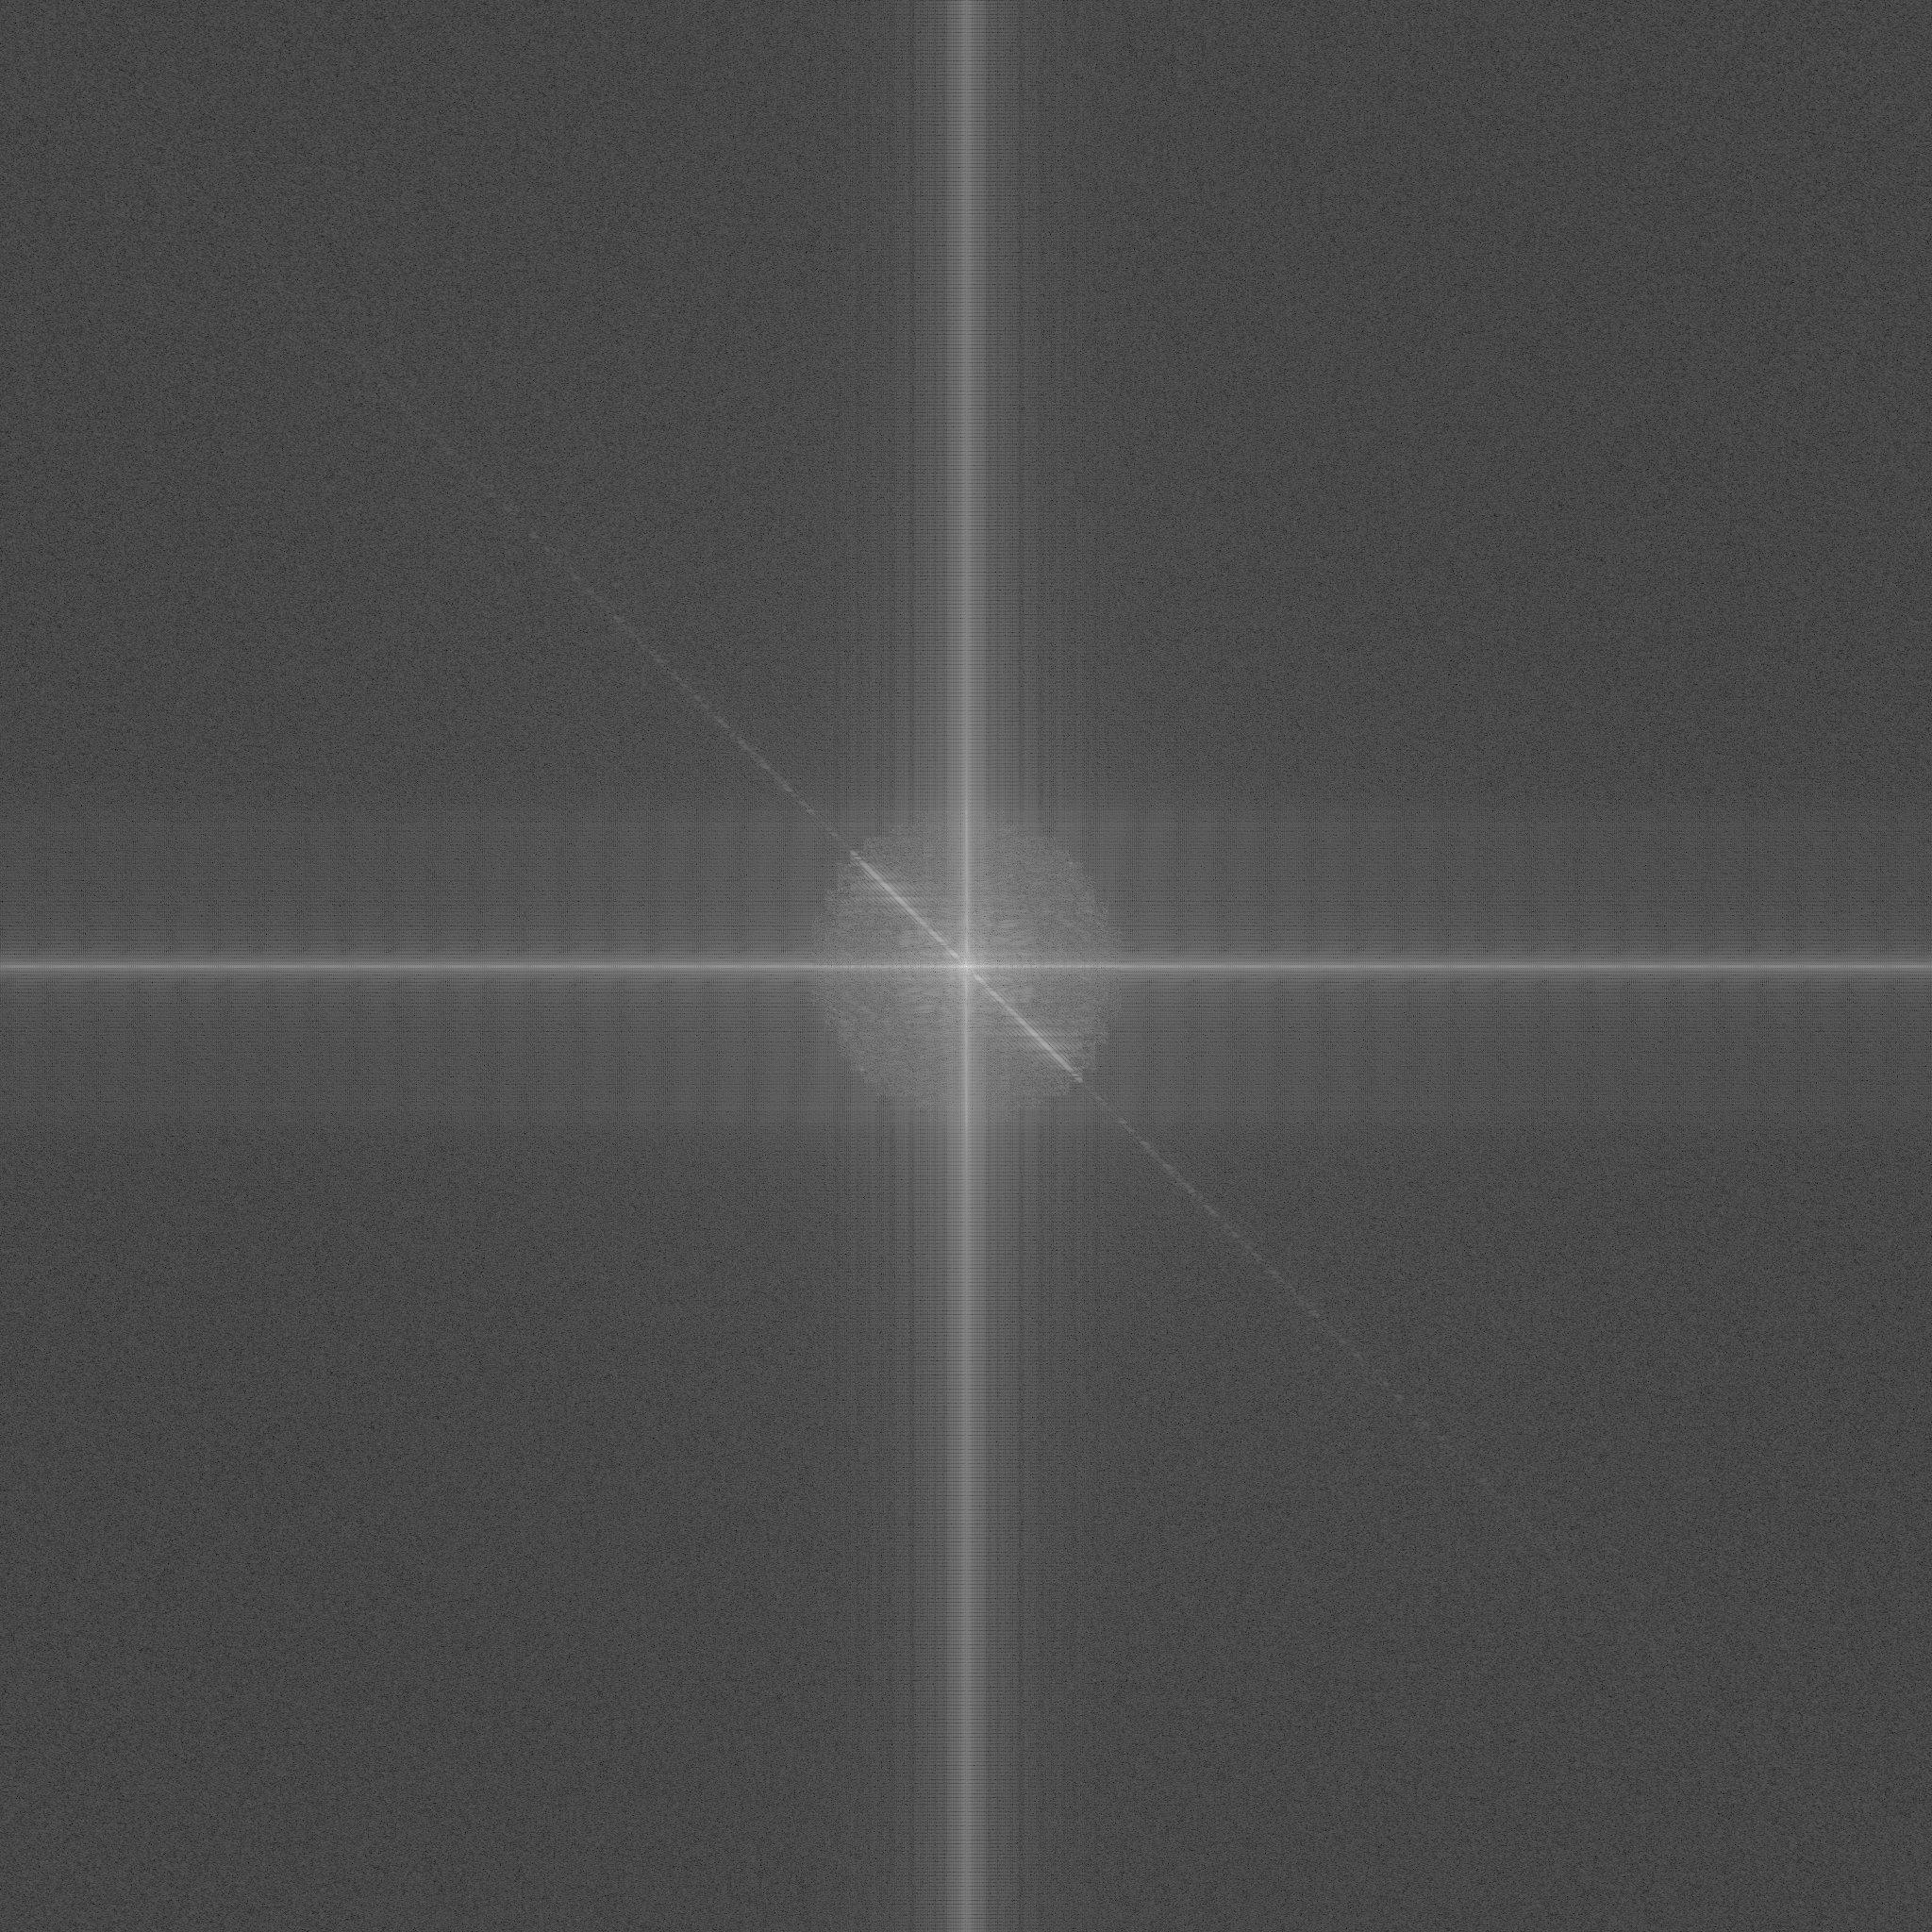
\includegraphics[height=2in]{./immagini_terza_prova/ex2/FFTofraw0_fft.jpg}}
  \caption{(a): original image. (b): gaussian filter transform of (a). (c): low-pass filter transform of (a). (d): FFT domain of (c).}
  \label{fig:ex_two}
\end{figure}

\begin{figure}[h]
	\centering
  \subfloat[][]{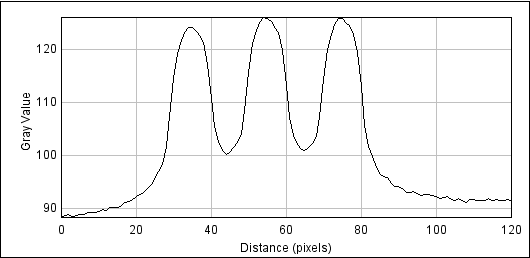
\includegraphics[height=1.15in]{./immagini_terza_prova/ex2/25_profile_histo_raw.PNG}}
  \subfloat[][]{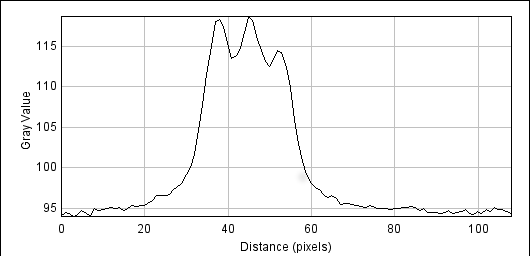
\includegraphics[height=1.15in]{./immagini_terza_prova/ex2/62_prof_histo_raw.PNG}}\\
  \subfloat[][]{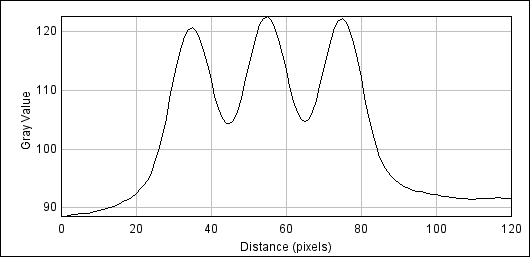
\includegraphics[height=1.15in]{./immagini_terza_prova/ex2/25_prof_histo_gaussian.PNG}}
  \subfloat[][]{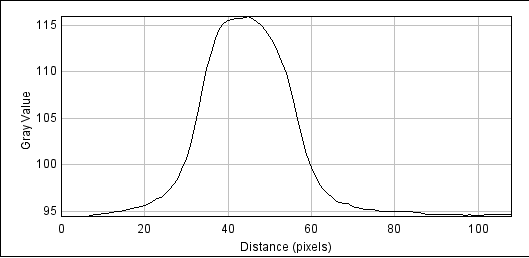
\includegraphics[height=1.15in]{./immagini_terza_prova/ex2/62_prof_histo_gaussian.png}}\\
  \subfloat[][]{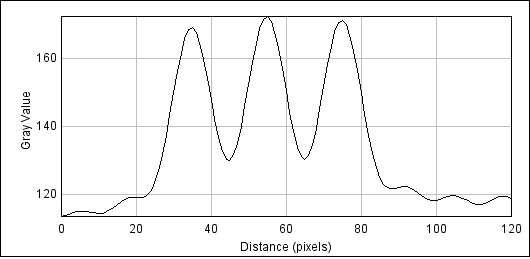
\includegraphics[height=1.15in]{./immagini_terza_prova/ex2/25_prof_histo_fft.PNG}}
  \subfloat[][]{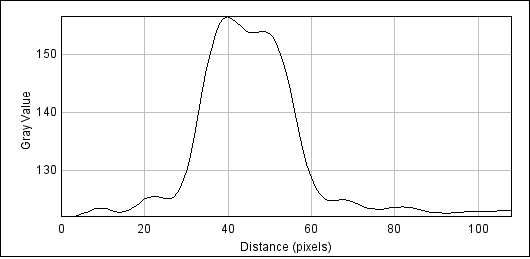
\includegraphics[height=1.15in]{./immagini_terza_prova/ex2/62_prof_histo_fft.PNG}}
  \caption{(From top to bottom) Averaged profile histogram of the raw picture for the $2.5\ lp/mm$ pattern (a) and $6.3\ lp/mm$ pattern (b); averaged profile histogram of the gaussian filtered picture for the $2.5\ lp/mm$ pattern (c) and $6.3\ lp/mm$ pattern (d); averaged profile histogram of the low-pass filtered picture for the $2.5\ lp/mm$ pattern (e) and $6.3\ lp/mm$ pattern (f)}
  \label{fig:ex_two_pro}
\end{figure}

The second exercise revolved around Fig. \ref{raw0}, which is affected by noise created during the acquisition process and contains various line patterns at different frequencies, measured in $lp/ mm$. Analog to what we did in Exercise 1, we were asked to reduce the noise through operations performed both in the spatial and frequency domains. In this case we were asked to evaluate the effect of the operations by calculating:
\begin{itemize}
\item SNR on a homogenous region, as defined in Exercise 1;
\item spatial resolution in terms of MTF which is defined as:
\begin{equation}
MTF=\frac{M_{out}}{M_{in}}=\frac{Modulation\ in\ recorded\ image}{Input\ modulation}
\end{equation}
where $M_{out}$ is given by the contrast in grey levels between the peaks and valleys of average profiles (the respective histograms, both for the raw and filtered image can be found in Fig. \ref{fig:ex_two_pro}) of the various line patterns, and $M_{in}$ is assumed to be equal to 40 gray levels in all cases. We decided to perform this operation for both the $2.5\ lp/mm$ and the
$6.3\ lp/mm$
\end{itemize}

\begin{table}[!htb]
	\centering
	\begin{tabular}{| l | l | l || l | l |}
		\hline
		Pattern      & Operation       & MTF           & Operation       & SNR \\ \hline
    $2.5\ lp/mm$ & raw             & $0.33 \pm 0.13$ & raw             & $20.95$ \\ \hline
                 & gaussian filter & $0.20 \pm 0.13$ & gaussian filter & $39.07$ \\ \hline
                 & low-pass filter & $0.50 \pm 0.13$ & low-pass filter & $39.99$ \\ \hline
    $6.3\ lp/mm$ & raw             & $0.08 \pm 0.12$ &                 & \\ \hline
                 & gaussian filter & $0.03 \pm 0.05$ &                 & \\ \hline
                 & low-pass filter & $0.05 \pm 0.05$ &                 & \\ \hline
	\end{tabular}
  \caption{Results of Exercise 2. Uncertainties on MTF, added due to the difficulty of performing a good measure by looking at the histogram, is computed using: $\delta MTF = \frac{\delta MTF_{out}*MTF}{MTF_{out}}$.}
  \label{tab:ex_two}
\end{table}

We decided to apply to the image a gaussian filter in the spatial domain and a low pass filter, the effect of which can be found in Fig.~\ref{fig:ex_two}. The SNR and MTF values are instead reported in Tab. \ref{tab:ex_two}. From the latter we can see that by reducing thenoise the SNR improves, while the spatial resolution decreases drastically due to the fact that contrast is diminished and the image gets blurred.



\section*{Exercise 3}

\begin{figure}[H]
	\centering
  \subfloat[][]{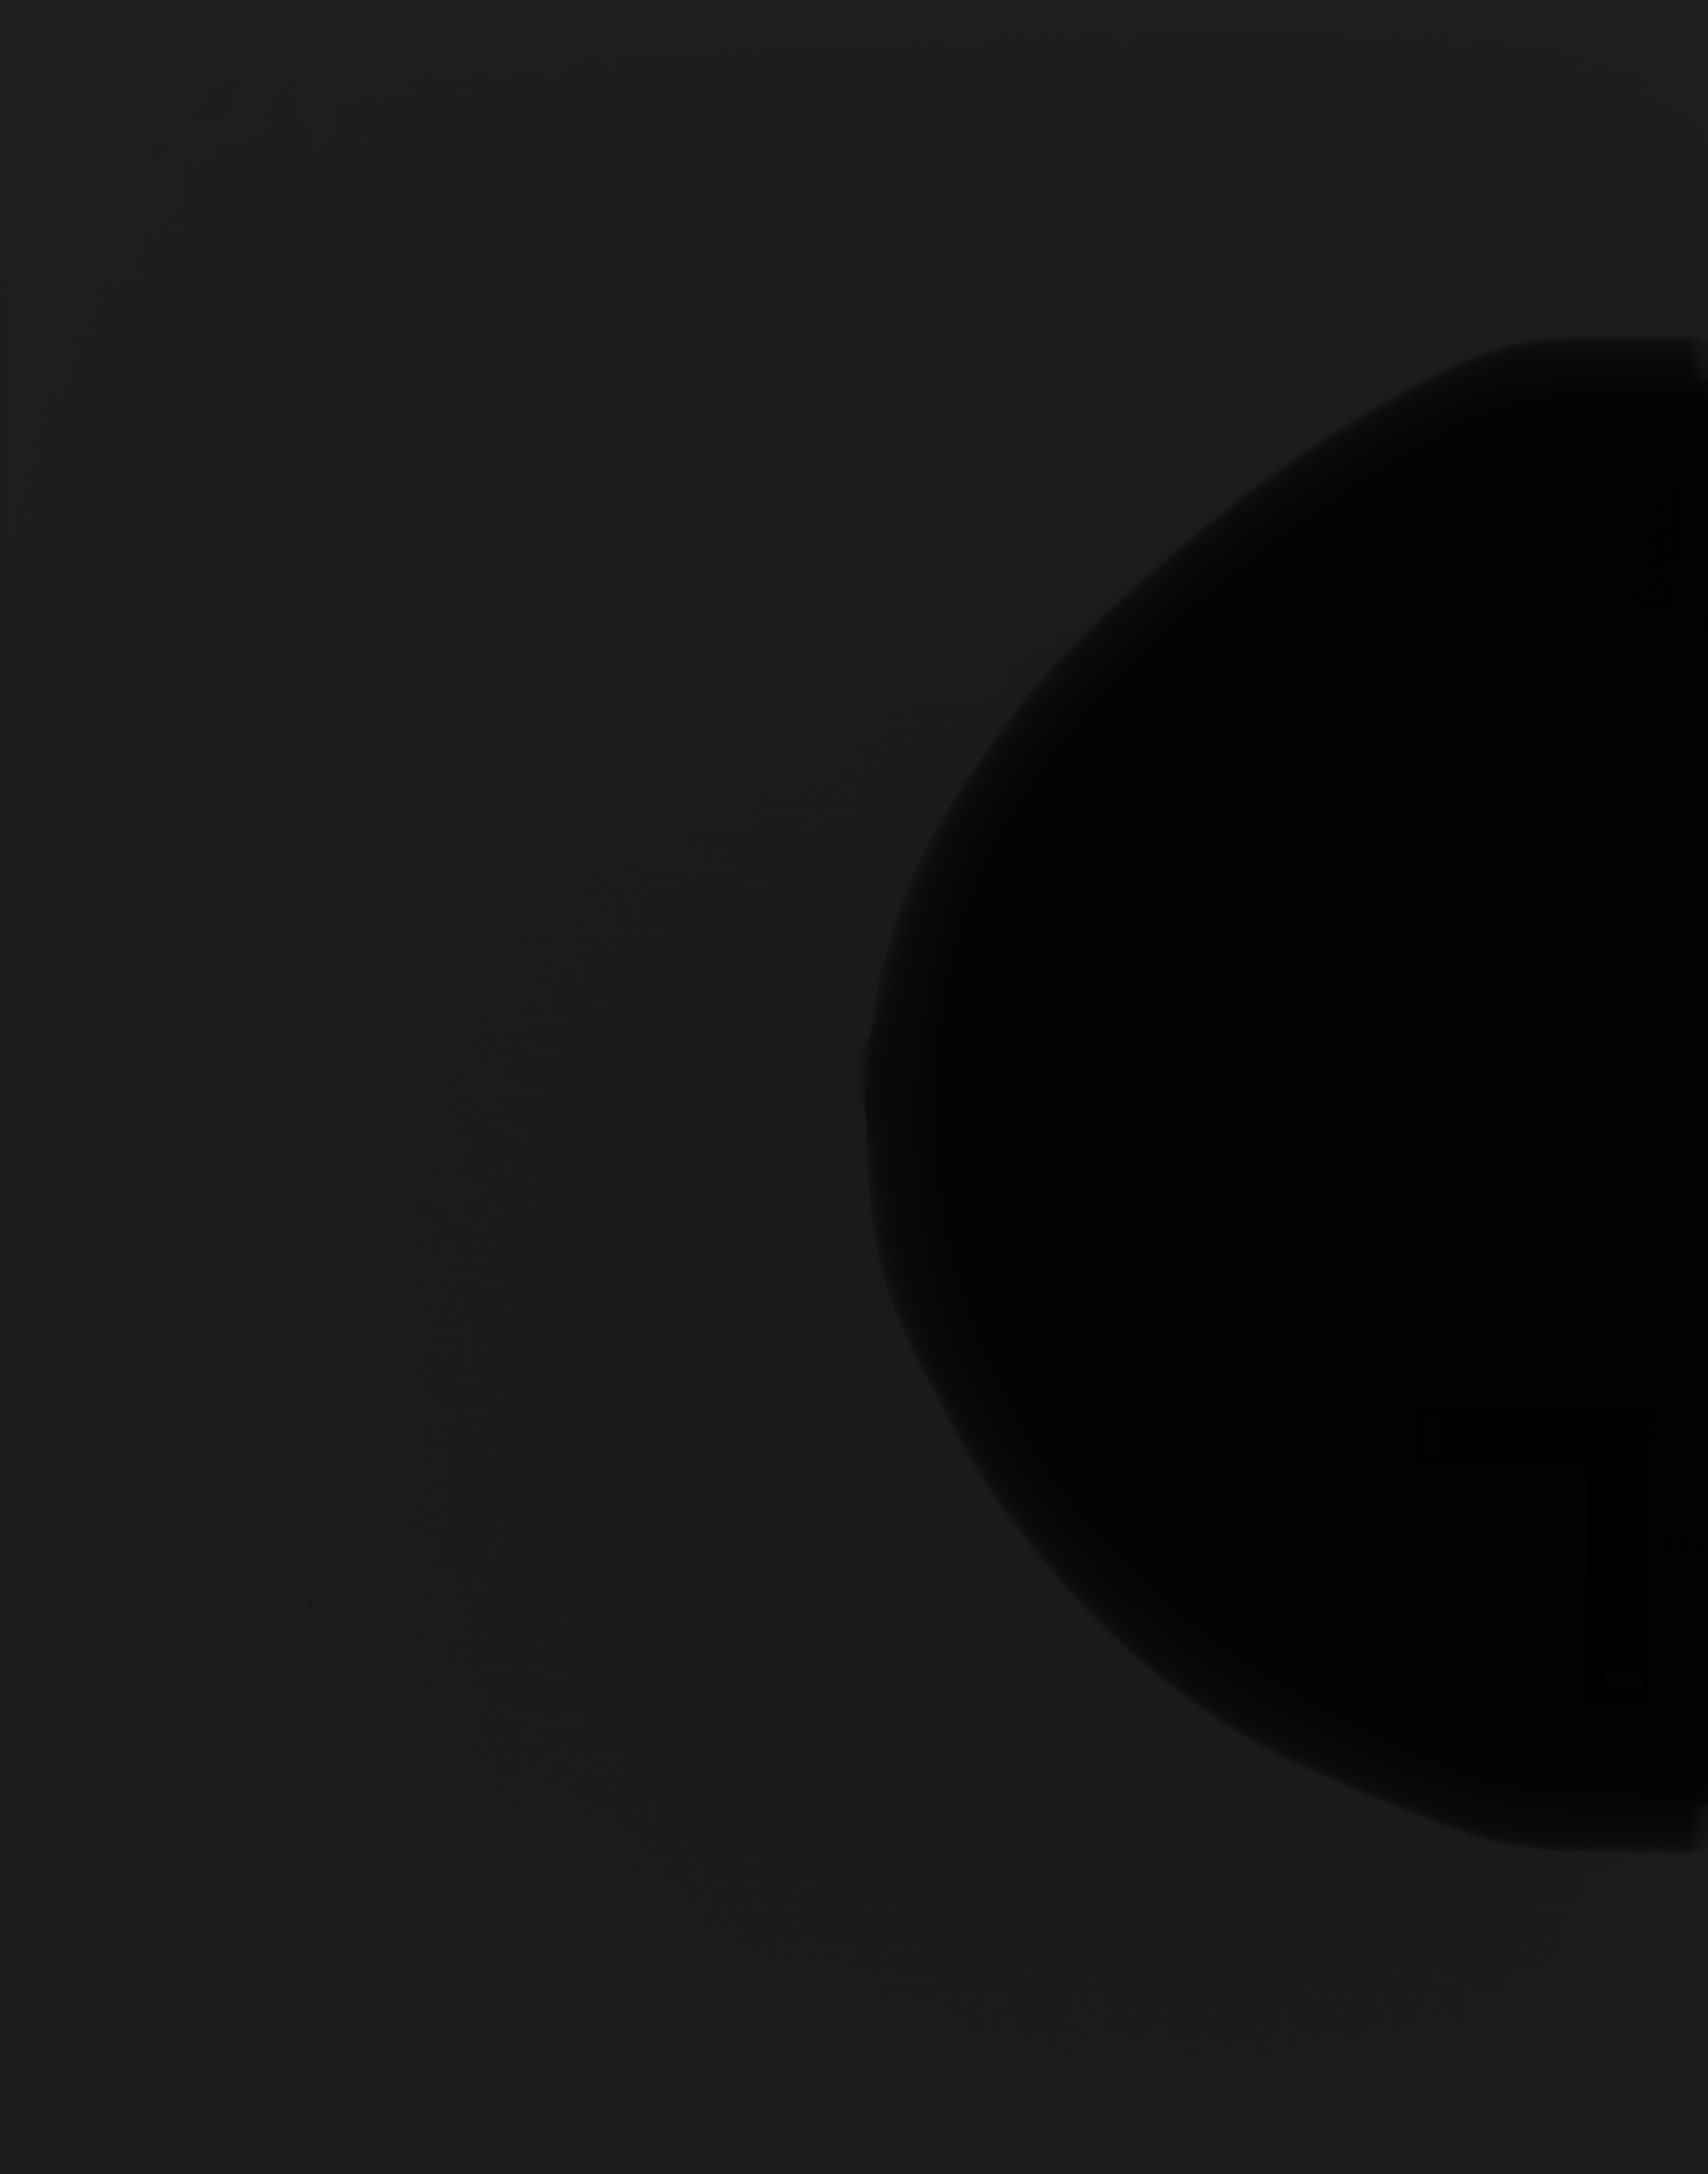
\includegraphics[width=.33\textwidth]{./immagini_terza_prova/ex3/cirs.jpg}\label{mammo_raw}}\quad
  \subfloat[][]{
\includegraphics[width=.33\textwidth]{./immagini_terza_prova/ex3/flat-field.jpg}\label{mammo_flatfield}}\\
  \subfloat[][]{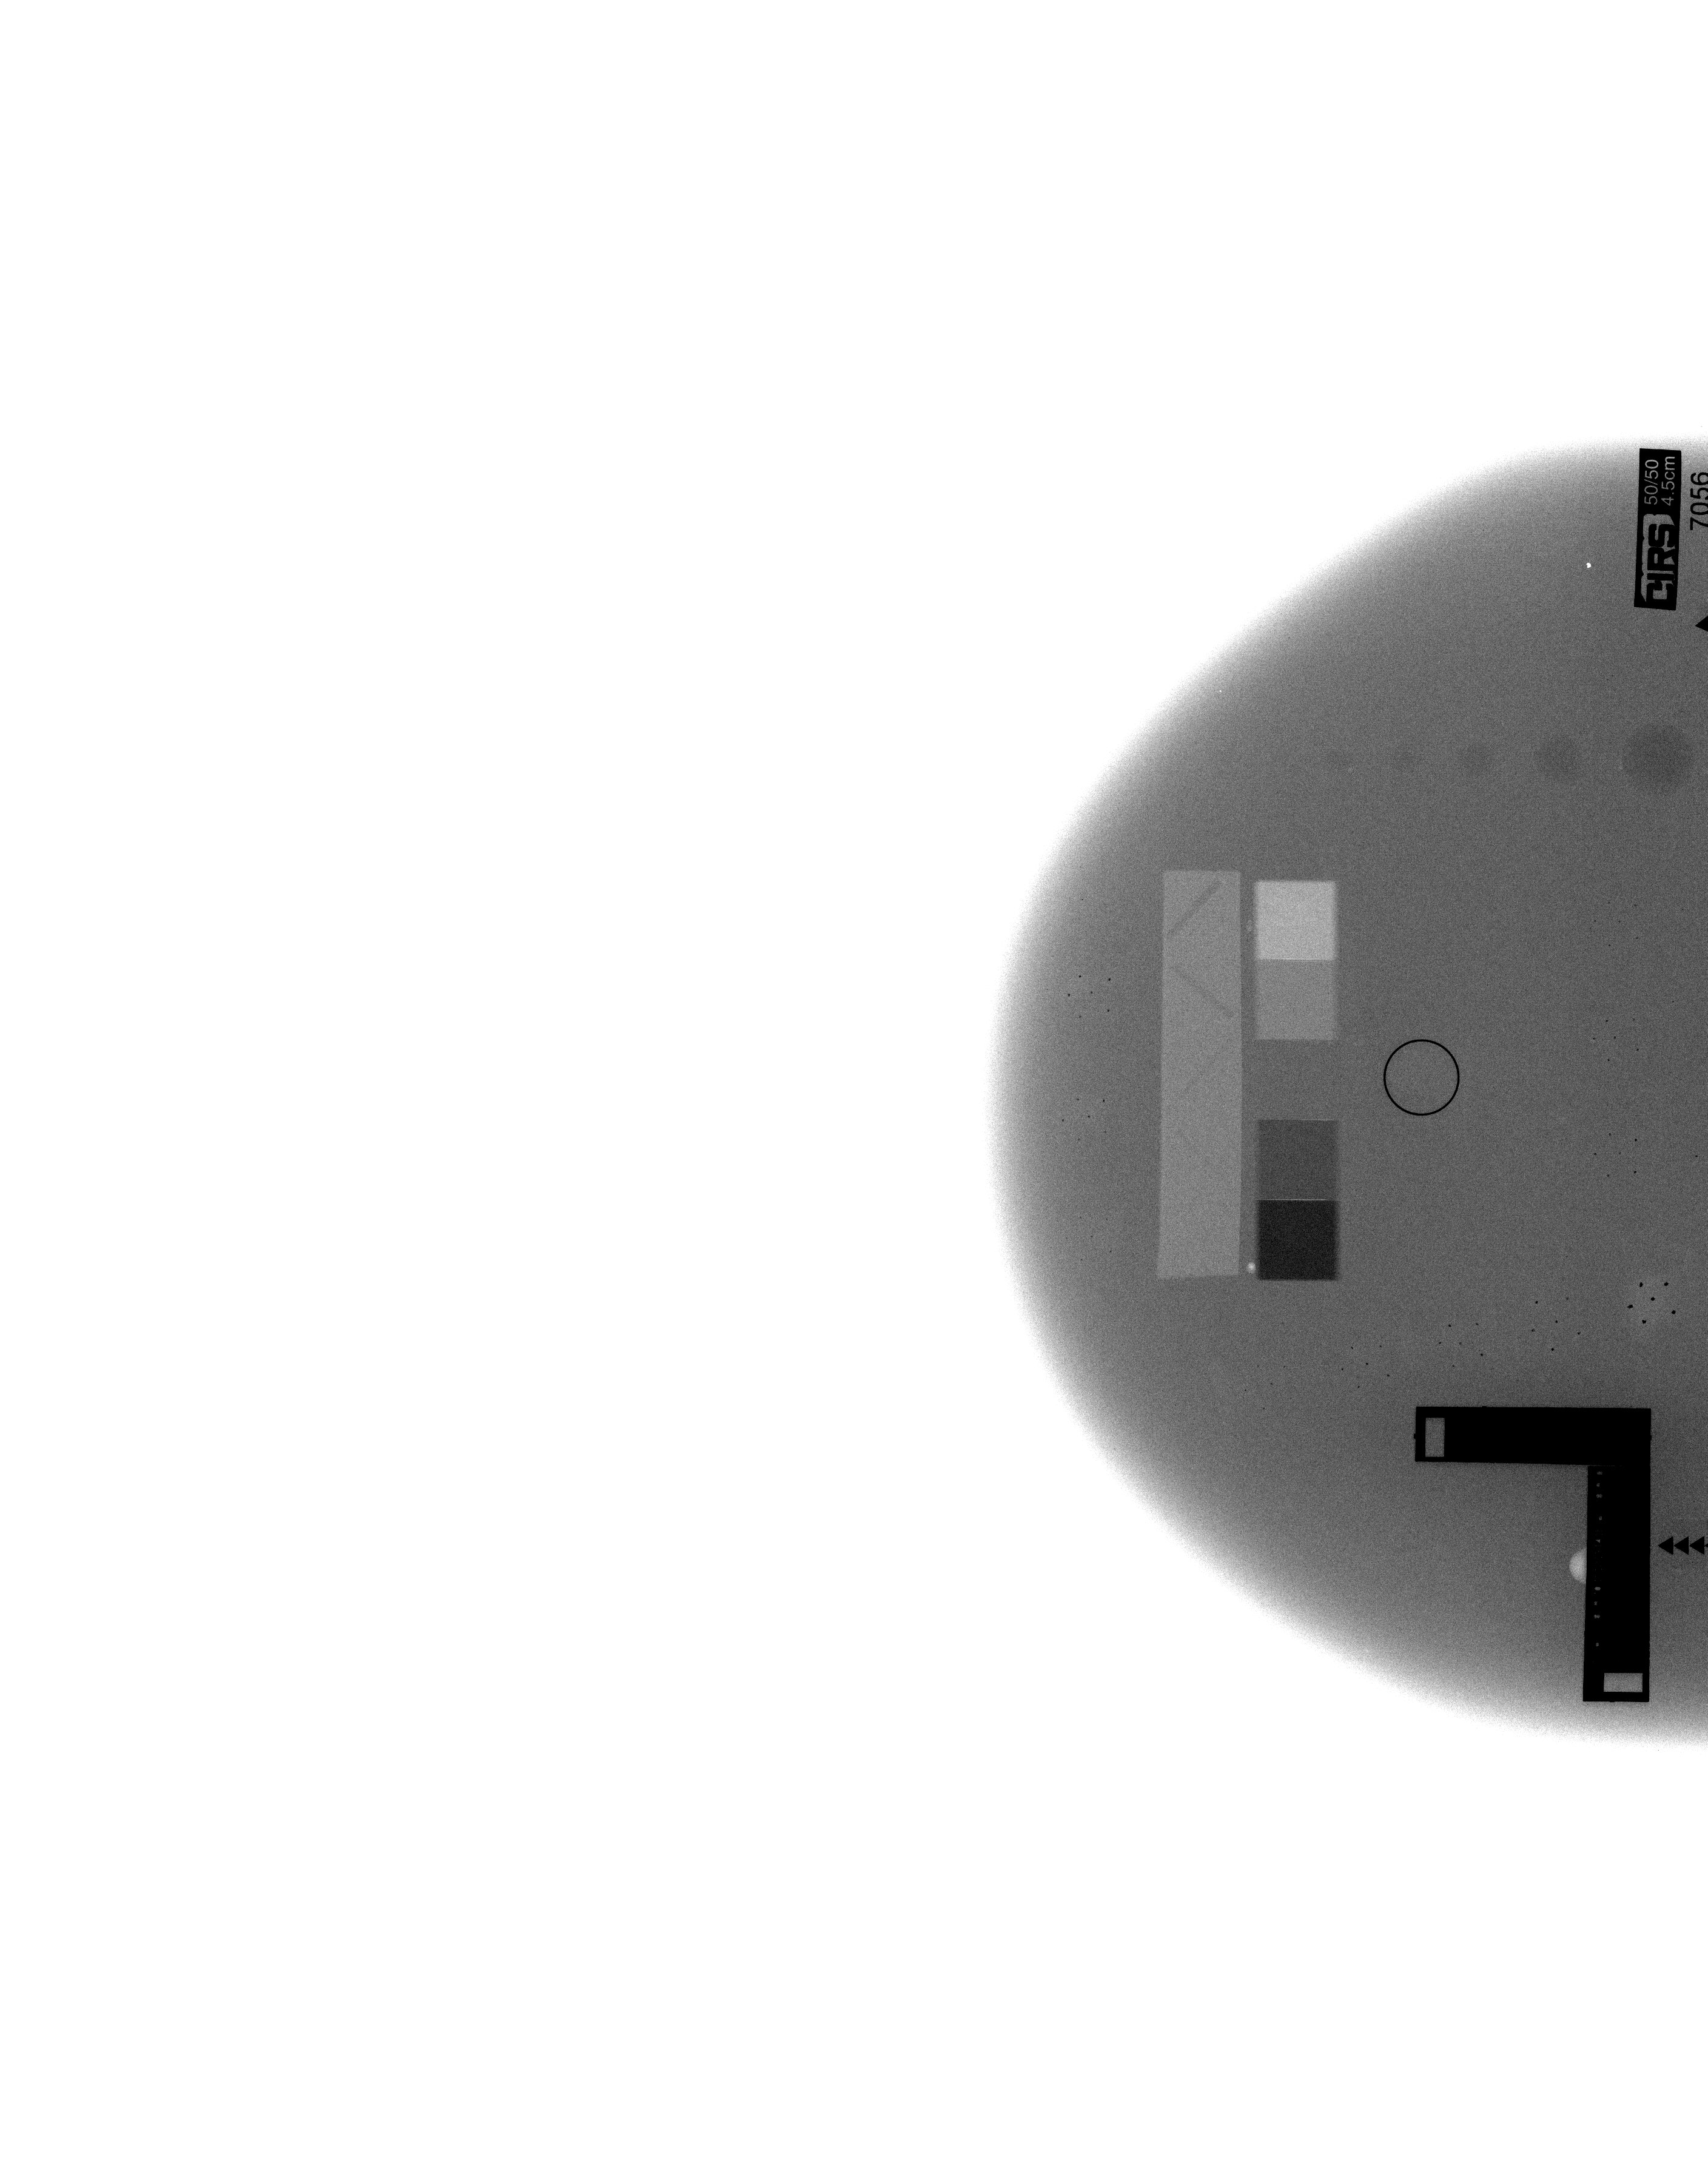
\includegraphics[width=.33\textwidth]{./immagini_terza_prova/ex3/Resultofcirs.jpg}\label{mammo_corrected}}
  \caption{(a): raw mammographic picture with circular details within the phantom. (b): flat-field image. (c): flat-field corrected image.}
  \label{fig:ex_three}
\end{figure}

For Exercise 3 we were asked to perform a flat-field correction on the mammographic image in Fig~\ref{fig:ex_three}. This operation can be performed by subtracting pixel by pixel a flat-field image from our raw image and multiplying by a normalization constant:
\begin{equation}
IC=(\frac{IR}{IF})* M
\end{equation}
where IC is the corrected image (Fig.~\ref{mammo_corrected}), IR is the raw image (Fig.~\ref{mammo_raw}), IF is the flat-field image (Fig.~\ref{mammo_flatfield}) and M is the normalization constant, which in this case is assumed to be equal to 100.
We were then asked to evaluate the image quality using:
\begin{itemize}
	\item profile and SNR on an extended area outside the phantom (as described in Exercise 1);
	\item CNR evaluated on the circular inserts within the phantom, by applying the formula:
	\begin{equation}
	CNR=\frac{I_{detail}-I_{background}}{\sigma_{background}}
	\end{equation}
	where $I_{detail}$ and $I_{background}$ are the averege gray level of the detail and a homogenous area of the phantom respectively and $\sigma_{background}$ is the gray level standard deviation for the same region, which can be interpreted as its noise. We calculated this parameter for two of the the details in the picture.
\end{itemize}

\begin{table}[h]
	\centering
	\begin{tabular}{| l | l | l | l | l |}
		\hline
		 Operation  & $\sigma_{profile}$ & SNR   & CNR(big detail) & CNR(small detail)\\ \hline
     Raw        & 178.07             & 38.32 & 1.77            & 1.05 \\ \hline
     Flat-field & 11.56              & 59.51 & 1.23            & 0.58 \\ \hline
	\end{tabular}
  \caption{Results of exercise 3.}
  \label{tab:ex_3}
\end{table}

The results of this operation are reported in Tab.~\ref{tab:ex_3}. From the latter we can see that SNR increases, being the noise reduced, while the CNR decreases due to the reduction of the difference between the intensities of details and background.

\clearpage

\section*{Exercise 4}


\begin{figure}[h]
	\centering
	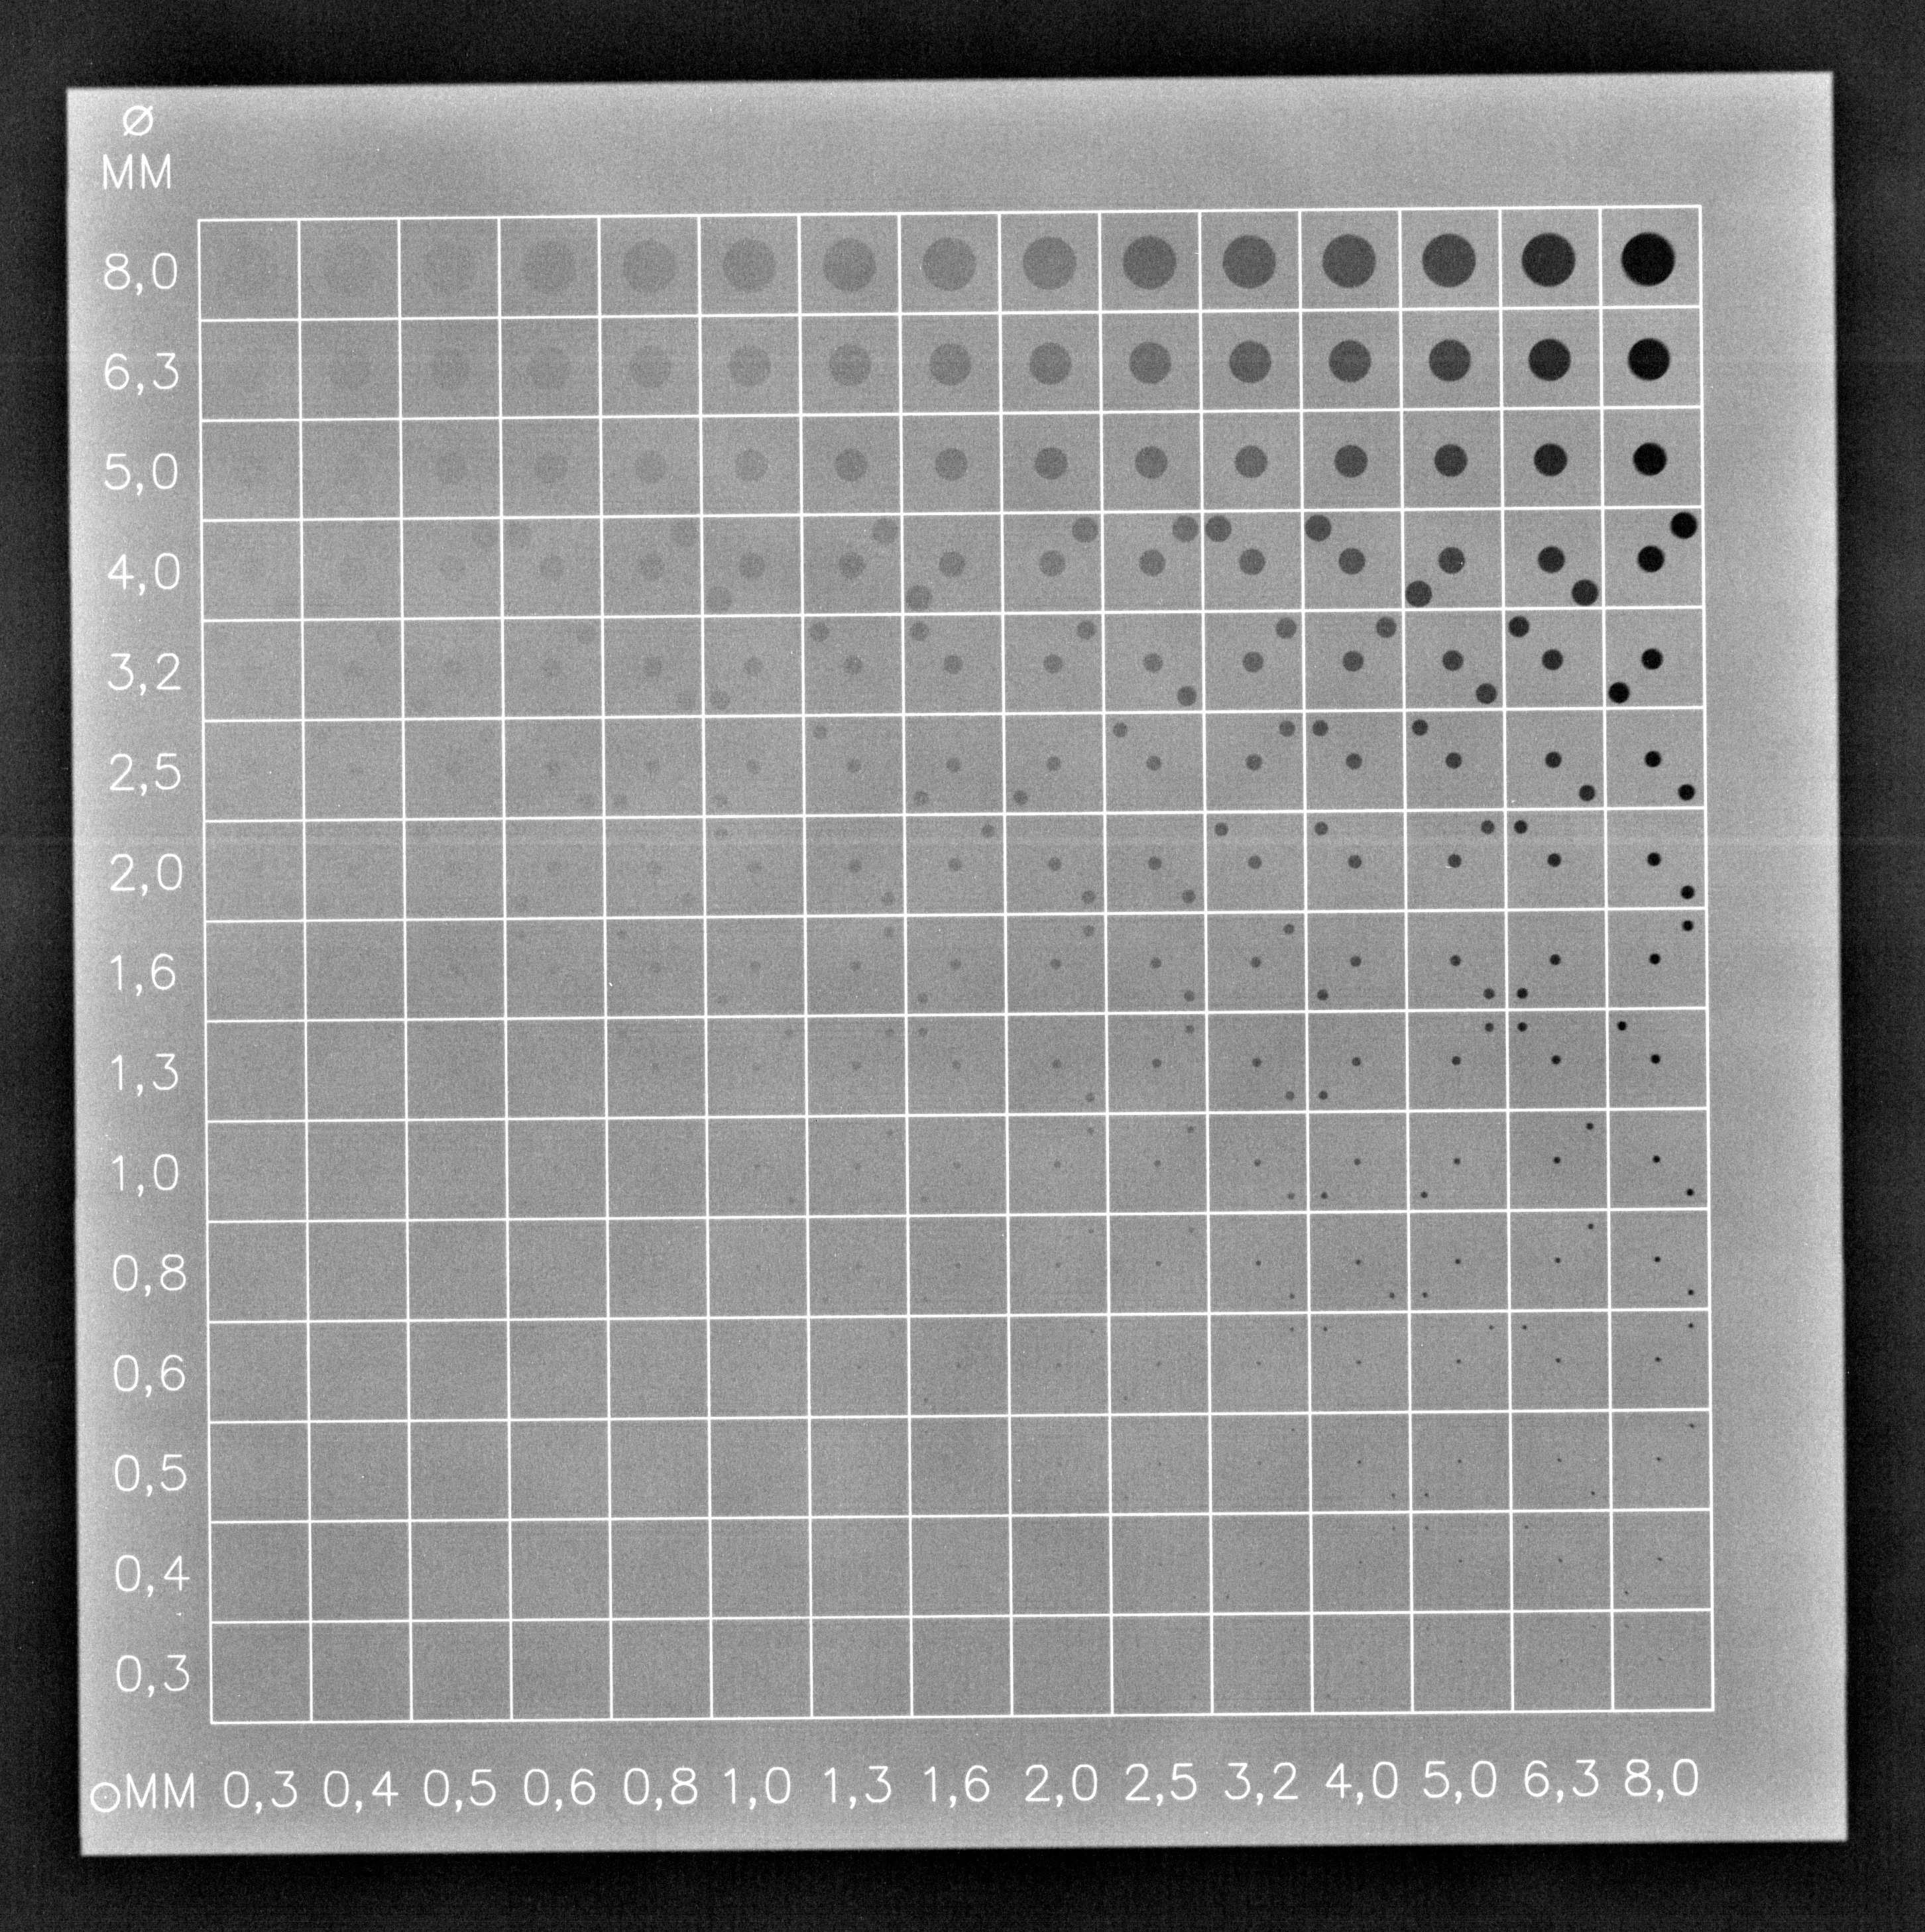
\includegraphics[width=0.8\textwidth]{./immagini_terza_prova/ex4/CDRAD-10_3.jpg}
  \caption{Picture of the phantom we used to evaluate the performance of the detection system.}
  \label{fig:phantom}
\end{figure}

For the last session of the experience we were asked to evaluate the performance of the detection system, through a contrast-detail analysis  performed on Fig.~\ref{fig:phantom}, which shows a picture (obtained with the detection system itself) of a table containing various circular shapes with different diameters (decreasing from top to bottom) and different levels of contrast with the background (decreasing from right to left).

\begin{figure}[!hbt]
	\centering
  \subfloat[][CNR as function of thickness, diameter of 2.5 mm.]{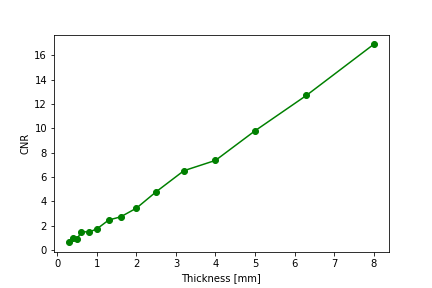
\includegraphics[width=.4\textwidth]{immagini_terza_prova/plots/25_plot.png}}\quad
  \subfloat[][CNR as function of thickness, diameter of 4.0 mm.]{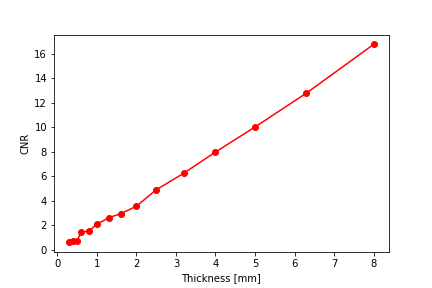
\includegraphics[width=.4\textwidth]{immagini_terza_prova/plots/4_plot.png}}\\
  \subfloat[][CNR as function of thickness, diameter of 6.5 mm.]{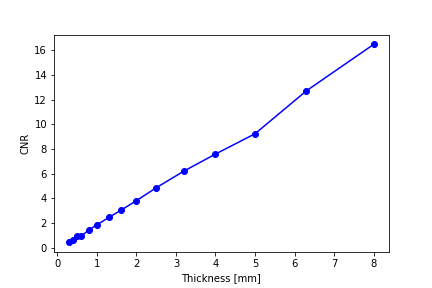
\includegraphics[width=.4\textwidth]{immagini_terza_prova/plots/65_plot.png}}\quad
  \subfloat[][CNR averaged over the thicknesses as a function of the diameter.]{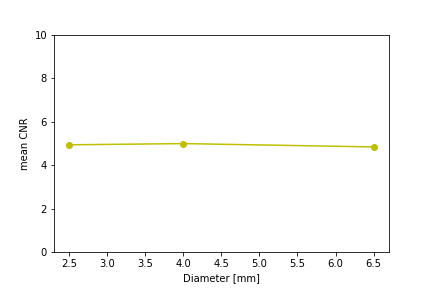
\includegraphics[width=.4\textwidth]{immagini_terza_prova/plots/dummy_plot.png}}
  \caption{Plots of the results of Exercise 4. We can see that for every diameter, CNR encreases more or less linearly with the details' thickness, while the mean is more or less the same for every thickness.}
  \label{fig:plots_ex4}
\end{figure}

To this end we calculated the CNR on the central detail for all cells relative to the three diameters: 6.3 mm, 4.0 mm and 2.5 mm. These values can be found graphed as a function of both thickness and diameter of the details in Fig.~\ref{fig:plots_ex4}.

\begin{table}[h]
	\centering
	\begin{tabular}{| l | l | l | l |}
		\hline
    Thickness [mm] & CNR, 2.5 mm & CNR, 4.0 mm & CNR, 6.5 mm\\ \hline
    8.0 & 16.88 & 16.75 & 16.47\\ \hline
    6.3 & 12.70 & 12.77 & 12.71\\ \hline
    5.0 & 9.79 & 10.01 & 9.22\\ \hline
    4.0 & 7.36 & 7.97 & 7.58\\ \hline
    3.2 & 6.51 & 6.24 & 6.21\\ \hline
    2.5 & 4.79 & 4.88 & 4.85\\ \hline
    2.0 & 3.44 & 3.55 & 3.80\\ \hline
    1.6 & 2.73 & 2.93 & 3.01\\ \hline
    1.3 & 2.47 & 2.61 & 2.44\\ \hline
    1.0 & 1.74 & 2.07 & 1.84\\ \hline
    0.8 & 1.48 & 1.54 & 1.43\\ \hline
    0.6 & 1.52 & 1.41 & 0.93\\ \hline
    0.5 & 0.88 & 0.74 & 0.96\\ \hline
    0.4 & 1.01 & 0.71 & 0.63\\ \hline
    0.3 & 0.65 & 0.61 & 0.44\\ \hline
	\end{tabular}
  \caption{CNR computed for three different diameters for all the detail thicknesses.}
  \label{tab:ex4}
\end{table}

The results are reported in Tab.~\ref{tab:ex4}.

\end{document}


